% Notes
%
%
%


\documentclass[11pt, a4paper, twoside]{article}
% Use UTF-8 input
\usepackage[utf8]{inputenc}

% Title, author, date
\title{Final project: simulation of a bubble column}
\author{Group 2:\\Gerasimos Chourdakis, Vasileios Magioglou}
\date{\today}

\usepackage{graphicx} % For graphics
\usepackage{fancyhdr} % Use fancy headers
\usepackage{siunitx} % Typeset SI units correctly
\usepackage{listings} % List code in the lstlisting environment
\lstset{numbers=left, showspaces=false, showstringspaces=false, frame=single}
 
% Define the fancy headers
\pagestyle{fancy}
\fancyhf{}
\fancyhead[RO,LE]{\small\thepage}
\fancyhead[LO]{\small Group 2: G. Chourdakis, V. Magioglou}% odd page header and number to right top
\fancyhead[RE]{\small Computational Thermo-Fluid Dynamics with Open Source Tools, final project}%Even page header and number at left top

\usepackage[bookmarks=true,pdfborder={0 0 0}]{hyperref} % hyperlinks in pdf
\usepackage{caption, subcaption} % subfigure environment

\usepackage{tabulary} % For tables with text wrapping

\usepackage[section]{extraplaceins} % do not move float objects out of section {made a change in package - have it in mind!}

\usepackage{amsmath}

% \usepackage[backend=biber,
% style=numeric,
% sorting=ynt]{biblatex}
% \addbibresource{bibliography.bib}

\begin{document}

\maketitle

\setcounter{tocdepth}{2}
\tableofcontents

\newpage

\section{Introduction}
In this project we simulated the flow inside a 3D, cylindrical bubble column using the application \texttt{bubbleFoam} of OpenFOAM. We studied different values for the diameter of the bubbles and the inlet velocity. Next, we simulated the interaction with an obstacle and we also studied some particular aspects and problems that we faced during our experiments. In this report, a quick introduction to the model is provided, as well as an extensive presentation of the setup of our case. This gave us a better understanding of the underlying phenomena and directions for further studying are presented at the end.

Please not that, apart from the results shown here, videos and demo cases can also be found in \href{https://tinyurl.com/gl4fhzo}{https://tinyurl.com/gl4fhzo} (hosted in our Dropbox).


\section{Physics, numerics and methodology}

\subsection{Numerical formulations of bubbleFoam}

The numerical solution of the two-phase equations relies on a segregated algorithm based on the PISO procedure extended to two-phase flows. The momentum equations are manipulated to stabilize the system of equation at the limits of the range of volume fractions, to avoid singularities. The details of the numerical methodology are briefly summarized below in the subsections. 

\subsubsection{Phase momentum equation}
The momentum equation is rewritten in non-conservative form to extract the volume fraction from the transport terms. Renaming the total stress tensor, decomposing it in a diffusive component and a correction term and also introducing the total phase velocity, the equation becomes:
\begin{align}
\begin{split}
\frac{\partial U_\mathrm{a}}{\partial t} & +U_\mathrm{a}^T\cdot \nabla U_\mathrm{a}-\nabla\cdot(v_\mathrm{a,eff}\nabla U_\mathrm{\phi})+\nabla\cdot R_\mathrm{\phi,eff}^C+\frac{\nabla\alpha_a}{\alpha_a}\cdot R_\mathrm{a,eff}^C = \\ 
&= -\frac{\nabla p}{\rho_a}+g+\frac{\alpha_\mathrm{b}}{\rho_\mathrm{a}}[A_d(U_b-U_a)+A_l+A_vm(\frac{dU_b}{dt}|_b-\frac{dU_a}{dt}|_a)]
\end{split}
\end{align}

The discretized equations can be represented as 
\begin{equation}
U_a=\frac{H_a}{A_a}-\frac{\nabla p}{\rho_a A_a}
\end{equation}

\begin{equation}
U_b=\frac{H_b}{A_b}-\frac{\nabla p}{\rho_b A_b}
\end{equation}

These equations will be used to correct the velocity after the pressure field is updated. 

\subsubsection{Phase continuity equation}
The phase continuity equations have to be solved ensuring that the phase fraction of each phase is kept between zero and one. To obtain this result, the dispersed phase continuity equation is rewritten as a function of the mean and relative velocity. Rewriting the phase velocity in terms of the relative velocity and the mean velocity weighted on the phase fractions we find 
\begin{equation}
U_a=U+a_b U_r
\end{equation}

Substituting into the phase continuity equation, a new expression is obtained 
\begin{equation}
\frac{\partial \alpha_a}{\partial t}+\nabla\cdot(\alpha_a U)+\nabla\cdot(\alpha_a(1-\alpha_a)U_r)=0
\end{equation}
which, if iteratively (Note that the equation is not linear) solved in a fully implicit manner, provides a bounded solution for the phase fraction field. 

\subsubsection{Pressure equation}
The pressure equation is obtained imposing that the divergence of the mixture flux is zero
\begin{equation}
\nabla\cdot\phi=\nabla\cdot(\alpha_\mathrm{a,f} \phi_a+\alpha_\mathrm{b,f} \phi_b)=0
\end{equation}

The phase fluxes are obtained by
\begin{equation}
\phi_a=\phi_a^*-\frac{1}{\rho_a A_a}|_f S_f\nabla p+\phi_\mathrm{dg,a}
\end{equation}

\begin{equation}
\phi_b=\phi_b^*-\frac{1}{\rho_b A_b}|_f S_f\nabla p+\phi_\mathrm{dg,b}
\end{equation}

\subsection{The bubbleFoam solver} \label{sec:bubbleFoam}
The solver bubbleFoam in OpenFOAM was selected to simulate the bubble column. This is based on theoretical study and testing of other solvers, e.g. twoPhaseEulerFoam. This section is largely drawn from openfoanwiki.net. The bubbleFoam solver is a two-phase solver based on the Euler-Euler two-fluid methodology, suitable to compute dispersed gas-liquid and liquid-liquid flows. In the Euler-Euler two-fluid approach, the phases are treated as interpenetrating continua, which are capable of exchanging properties, like momentum, energy and mass one with the other. Typical applications of the two-fluid approach, as implemented in bubbleFoam, are bubble columns, stirred tank reactors, static mixers etc.

The solution procedure adopted in the bubbleFoam solver is summed up as follows:
\begin{enumerate}
    \item{Solve the phase continuity equations}
    \item{Update lift, drag and virtual mass coefficients}
    \item{Construct the momentum equation matrix}
    \item{Predict the phase velocity fields, without considering the pressure gradient at this stage}
    \item{Solve the pressure equation}
    \item{Correct the velocities with the new pressure field, and update the phase fractions}
    \item{Solve the transport equations for the turbulence quantities}
\end{enumerate}

The structure of a typical bubbleFoam case is represented in the following directory tree shown in figure~\ref{fig:bubblefoamstructure}, which lists the directories and the files contained in the bubbleColumn tutorial. 
\begin{figure}[!ht]
 \centering
    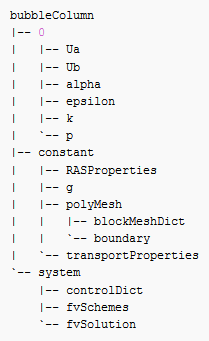
\includegraphics[width=50mm,scale=0.5]{figures/bubblefoamstructure.png}
    \caption{bubbleFoam case setup and structure}
    \label{fig:bubblefoamstructure}
\end{figure}

\subsubsection{bubbleFoam capabilities} \label{sec:bubbleFoamcapabilities}
The bubbleFoam solver implements the equations that are presented in the following, for the simulation of gas-liquid flows. The model undergoes the following assumptions:
\begin{itemize}
    \item{Phases are incompressible}
    \item{The dispersed phase particle diameter is constant}
    \item{The flow is isothermal}
    \item{Only momentum exchange is accounted for in the momentum transport equations}
\end{itemize}

The main features of the solver are the following:

\begin{itemize}
    \item{Capability to solve for dispersed two-phase flows with strong density ratio}
    \item{Robust solution algorithm, able to deal with complete flow separation}
    \item{Turbulence modelling through $k-\epsilon$ model and standard wall functions}
\end{itemize}

\subsubsection{bubbleFoam limitations} \label{sec:bubbleFoamlimitations}
The bubbleFoam solver currently has the following limitations:

\begin{itemize}
    \item{Only one dispersed phase and a continuous phase can be described. It is not possible to account for multiple dispersed phases (i.e. represent a dispersed phase diameter distribution)}
    \item{The diameter of the particles constituting the dispersed phase is assumed to be constant. Aggragation, breakage and coalescence phenomena are not accounted for}
    \item{The drag coefficient is computed as a blend of the drag coefficients evaluated for each phase on the basis of the phase fractions, and no alternative drag models are available}
    \item{The interaction between the phases happens only through the momentum exchange term in the corresponding momentum equations:}
    \begin{itemize}
        \item{It is not possible to model the heat transfer between the phases}
        \item{It is not possible to model the mass transfer between the phases}
        \item{No chemical reaction model is available}
        \end{itemize}
\end{itemize}

\subsection{Alternative solvers}
There are alternative solvers to be used for the simulation of a bubble column. Some of these are the twoPhaseEulerFoam, which we implemented as an additional test case and the interFoam provided by OpenFOAM.

\subsubsection{twoPhaseEulerFoam solver}
Two incompressible fluid phases with one phase dispersed are solved using this solver. Both the phases are described using the Eulerian conservation equations and thus it is referred  as  Euler-Euler model. Each of the phases are treated as a continuum in this approach. This solver is considered an extension of the bubbleFoam solver. It offers the option of particle-particle interactions, as well as more drag models to choose from to estimate the drag coefficients for each phase.
In comparison to the bubbleFoam solver structure, it includes three additional files in the constant folder which help in setting different models and properties for simulating two phase flows (InterfacialProperties, kineticTheoryProperties, ppProperties). There is also an extra boundary condition in the 0 folder, called Theta and represents the granular temperature. 

\subsubsection{interFoam solver}
According to "OpenFOAM User Guide" interFoam is a solver for 2 incompressible fluids, which tracks the interface and includes the option of mesh motion. It uses the multidimensional universal limiter for explicit solution (MULES) method, created by OpenCFD, to maintain boundedness of the phase fraction independent of underlying numerical scheme, mesh structure, etc. The choice of schemes for convection are therefore not restricted to those that are strongly stable or bounded, e.g. upwind differencing. We have not implemented interFoam for bubbleColumns, but still remains an option for this type of simulations.

\subsubsection{MPPICInterFoam solver}
The new MPPICInterFoam solver combines Multi-Phase Particle In Cell (MP-PIC) Lagrangian cloud modelling for particles with high volume loading, with two phase isothermal and immiscible fluids modelling using Volume of Fluid (VOF) interface capturing. Particles are modelled using the same approach adopted in the MPPICfoam solver, including the effect of the volume fraction of particles on the continuous phase. To limit the particles crossing the interface, typically from liquid to gas, a new interface force was introduced. This force acts in the direction normal to the interface and only near the interface according to the expression 

\begin{equation}
F_\mathrm{interface} = Cm\nabla(a_w)
\end{equation}
where ${m}$ is the particle mass, ${a_w}$ the liquid volume fraction, and ${C}$ a model coefficient. These are specified in the particleForces sub-dictionary of the cloudProperties file. The solver includes support for Multiple Reference Frame (MRF) forces, specified via the MRFProperties file, and other forces via fvOptions. Turbulence modelling is generic, supporting RAS, LES/DES or laminar models. 

We discovered this solver recently after the completion of our project. It was released in June 2016. It seems like a promising improved solver to simulate two phases in particular bubble columns, while at the same time it offers enhanced visualization effects for the discrete separation of the phases.




\section{Setup}

\subsection{Starting point}
We designed our case based on the \emph{bubbleColumn} tutorial of the \texttt{bubbleFoam} solver, of OpenFOAM version 2.0.1. An example of the results of this tutorial is shown in figure~\ref{fig:bubbleColumn_tutorial}. This is a 2D case that uses a uniform grid and sets a continuous air inlet from the whole area of the bottom boundary. We wouldn't expect to observe individual bubbles but, eitherways, these rough results don't help us much to understand the phenomena that take place.

\begin{figure}
    \centering
    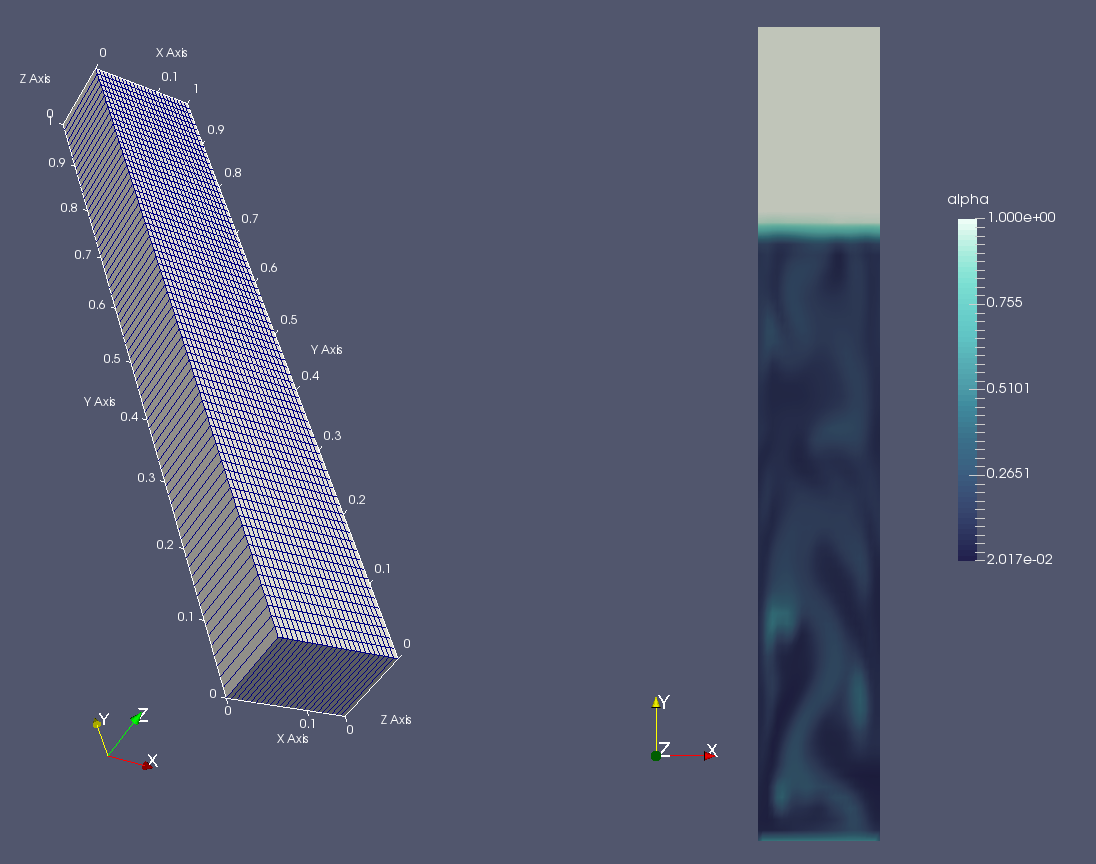
\includegraphics[width=\textwidth]{figures/bubbleColumn_tutorial}
    \caption{\emph{bubbleColumn} tutorial of the solver \texttt{bubbleFoam}, used as a base for our project. A pseudo-2D uniform grid is used, with continuous air inlet from the whole bottom boundary. The size of bubbles introduced is $d_\mathrm{a}=\SI{3}{\milli\metre}$ and the inlet velocity $U_{\mathrm{a},y}=\SI{0.1}{\metre/\second}$.}
    \label{fig:bubbleColumn_tutorial}
\end{figure}

We extended this case to simulate the introduction of the air only through a small hole at the bottom and with pulses. This gave us structures that behaved like bigger bubbles. We will refer to these simply as ``bubbles'' in the rest of the text, except if noted differently. We also transferred the problem from 2D to 3D, creating a coarse cylindrical mesh and refining in the most active areas. Furthermore, we introduced obstacles and explored different inlet scenarios.

\subsection{Mesh setup and refinement}
In our case we used a cylindrical mesh, created with \texttt{blockMesh} and partially refined with \texttt{refineMesh}. The full-size mesh ($h=\SI{0.5}{\metre}$) for our main case is shown in figure~\ref{fig:main_mesh} and a fraction of the source \texttt{blockMeshDict} is shown in listing~\ref{lst:blockMeshDict}. The mesh is constructed by five blocks, i.e. one central pillar and four peripheral blocks. The edges of the blocks are of type \texttt{arc}. All the blocks have the same number of cells, but the central pillar is smaller and therefore denser.

The mesh is then partially refined using the tools \texttt{setSet} and \texttt{refineMesh}. Two areas are of specific interest: the central pillar in which the bubbles are expected to travel and the volume around the interface with the atmosphere. These are defined in the file \texttt{refine.setSet}, as shown in listing~\ref{lst:refine.setSet}. The refinement in done one time (splitting to two) towards all the three directions, as set in the \texttt{refineMeshDict} (not listed here).

\begin{figure}
    \centering
    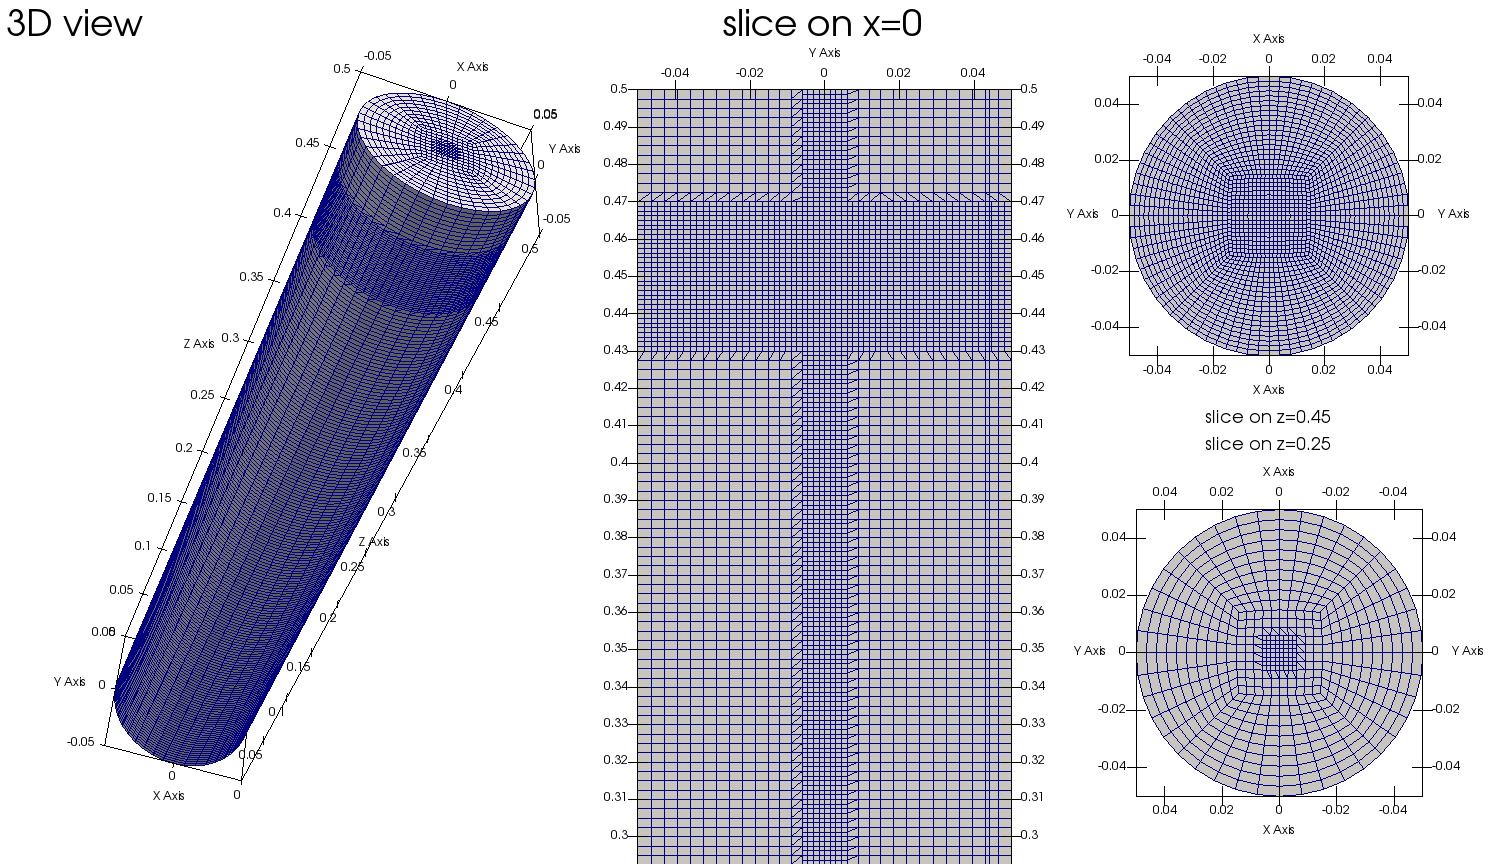
\includegraphics[width=\textwidth]{figures/main/mesh_print.png}
    \caption{Mesh for the main case: 3D cylinder of $\SI{0.50}{\metre}$ length and $\SI{0.10}{\metre}$ diameter. The base mesh (without refinement) consists of 200 cells in the $z$ direction and 30 cells towards the $x$ and $y$ directions. Two zones are refined once (the cell size is halved): a symmetric rectangular central pillar with width $\SI{0.01}{\metre}$ and the volume of the cylinder between $z=\SI{0.43}{\metre}$ and $z=\SI{0.47}{\metre}$. These parts correspond to the expected ``bubble'' lift volume and a zone around the interface with the atmosphere. In total, the mesh consists of 228\,360 cells. The flow direction is set towards the positive $z$.}
    \label{fig:main_mesh}
\end{figure}

\begin{lstlisting}[language=C++, caption={Fraction of the \texttt{blockMeshDict} used in the main case.}, label={lst:blockMeshDict}]
// 16 vertices (8 per z): on each z-face, 
// an outer and an inner square
vertices
(
    (-3.535534e+01 -3.535534e+01 0.000000e+00) // 0
    ...
    (-1.414214e+01  1.414214e+01 0.5000e+03) // 15
);

// 5 blocks: a central pillar and 4 peripheral
blocks
(
hex (0 1 5 4 8 9 13 12)   pipe (10 10 200) 
  edgeGrading (1.000000 ...[11 times])
...
hex (4 5 6 7 12 13 14 15) pipe (10 10 200) 
  edgeGrading (1.000000 ...[11 times])
);

// 16 arc-time edges for the inner and outer "circles"
edges
(
arc 0 1 (-9.184851e-15 -5.000000e+01 0.000000e+00)
...
arc 15 12 (-1.500000e+01 1.836970e-15  0.5000e+03)
);

patches
(
patch wall(...)
patch bottom(...)
patch atmosphere(...)
);
\end{lstlisting}

\begin{lstlisting}[language=C++, caption={\texttt{refine.setSet} file to select the cells to be refined.}, label={lst:refine.setSet}]
# Central pilar
cellSet toBeRefined new boxToCell 
  ( -0.005 -0.005 0.0 ) ( 0.005 0.005 0.5 )

# Interface with the atmosphere
cellSet toBeRefined add boxToCell 
  ( -0.05 -0.05 0.40 ) ( 0.05 0.05 0.5 )
\end{lstlisting}

In the case of the obstacle (figures~\ref{fig:obstacle_overview} and~\ref{fig:obstacle_colored}), another iteration of refinement is done for the area around the introduced obstacle (before it gets introduced), as set in a similar \texttt{refineSphere.setSet} file. The volume of the obstacle is then selected again with the \texttt{setSet} tool, using the \texttt{obstacle.setSet} file shown in listing~\ref{lst:obstacle.setSet} and removed using the \texttt{subsetMesh} tool to overwrite the initial mesh. An alternative approach would have been to use the \texttt{snappyHexMesh}, that would also change the shape of the cells around the object. We chose this method as it was simpler since we were already working with \texttt{blockMesh}. The exact way of calling these tools can be found in the \texttt{Allrun}, \texttt{Allparrun}, \texttt{Allparrun\_job} of the demo cases.

\begin{lstlisting}[language=C++, caption={\texttt{obstacle.setSet} file to select the cells to be removed (obstacle).}, label={lst:obstacle.setSet}]
cellSet wallObstacle new
cellSet wallObstacle invert

cellSet wallObstacle delete sphereToCell 
  (0.0 0.0 0.05) 0.005
\end{lstlisting}

\subsection{Initial and boundary conditions}
In the \texttt{blockMeshDict} (listing~\ref{lst:blockMeshDict}) the following patches are defined: \texttt{wall}, i.e.\@ the cylinder that encapsulates the domain (and the sphere, in the case of the obstacle), \texttt{bottom}, i.e.\@ the bottom wall (the same as \texttt{wall}, but can be treated differently if desired to do so) and \texttt{atmosphere}, i.e.\@ the top boundary that connects to the outer world. An additional patch is created for the inlet, named \texttt{bubble}, using the \texttt{setSet} and \texttt{createPatch} tools. The configuration file is shown in listing~\ref{lst:makeFaceSet.setSet}. The \texttt{createPatchDict} is not listed here. 

The initial and boundary conditions are shown in table~\ref{tab:bc_main}. The \texttt{alpha} is initialized to be 0 (continuous phase) at the bottom of the column and 1 (dispersed phase) at the top of the column. This is done with the \texttt{setFields} tool, using the \texttt{setFieldsDict} shown in listing~\ref{lst:setFieldsDict}. At the inlet, it is set to be either 0 or 0.95, using a \texttt{groovyBC} with the condition \texttt{mag(Ua) > 0}. We observed in our early experiments that a non-pure inlet stream was helping the stability of the solution. On the walls and on the top boundary the \texttt{alpha} is simply set to not change.

The velocities \texttt{Ua} and \texttt{Ub} are initialized to zero and no-slip walls are assumed. For the atmosphere, an \texttt{inletOutlet} boundary condition is used in both cases. At the inlet the water velocity is always set to zero, while the air velocity varies with time. For this, the \texttt{timeVaryingUniformFixedValue} boundary condition is used, which requires the OpenFOAM version 2.0.1 (it doesn't work with the v.2.1.1 that is the default in the computer lab). The file \texttt{Ua\_time.dat} provides the pattern, as shown in listing~\ref{lst:Ua_time.dat}, that is repeated.

The pressure \texttt{p} is initialized to $10^{-5}$ and the same value is set for the atmosphere (outlet), as required for compressible flows. On the walls, the gradient is set to zero using \texttt{buoyantPressure}. On the inlet, \texttt{zeroGradient} is used. The former corresponds to the static pressure and was used in the tutorial. The latter was chosen by us and we didn't face any problems.

\begin{lstlisting}[language=C++, caption={\texttt{makeFaceSet.setSet} file to select the inlet cells.}, label={lst:makeFaceSet.setSet}]
faceSet fbubble new boxToFace 
  (-0.002 -0.002 -0.0001) (0.002 0.002 0.0001)
\end{lstlisting}

\begin{table}
\centering
\begin{tabulary}{\linewidth}{L|lll}
\hline
\textbf{Field} & \textbf{Scope} & \textbf{Type/Value} & \textbf{Notes}\\
\hline
    gas fraction & initial & 0 or 1 & \texttt{setFields}\\ 
    (\texttt{alpha}) & bubble & 0 or 0.95 & \texttt{groovyBC}\\
                     & atmosphere & \texttt{zeroGradient} & -\\
                     & wall   & \texttt{zeroGradient} & -\\
    \hline
    air velocity  & initial & (0 0 0) & -\\
    (\texttt{Ua}) & bubble & 0 or (0 0 0.2) & time varied\\
                  & atmosphere & \texttt{inletOutlet} 0 0 & (0 0 0)\\
                  & wall & (0 0 0) & -\\
    \hline
    water velocity& initial & (0 0 0) & -\\
    (\texttt{Ub}) & bubble & (0 0 0) & -\\
                  & atmosphere & \texttt{inletOutlet} 0 0 & (0 0 0)\\
                  & wall & (0 0 0) & -\\
    \hline
    pressure      & initial & $10^{-5}$ & -\\
    (\texttt{p})  & bubble & \texttt{zeroGradient} & -\\
                  & atmosphere & $10^{-5}$ & -\\
                  & wall & \texttt{buoyantPressure} 0 & -\\
\hline
\end{tabulary}
\caption{Initial and boundary conditions for the main case.}
\label{tab:bc_main}
\end{table}

\begin{lstlisting}[language=C++, caption={\texttt{setFieldsDict} file to partially fill the column.}, label={lst:setFieldsDict}]
defaultFieldValues(
    volScalarFieldValue alpha 1
);

regions(
    boxToCell {
        box (-0.05 -0.05 0) (0.05 0.05 0.45);
        fieldValues(volScalarFieldValue alpha 0);
    }
);
\end{lstlisting}

\begin{lstlisting}[language=C++, caption={Time pattern of the \texttt{Ua} at the inlet}, label={lst:Ua_time.dat}]
(
  (0.000 (0 0 0.2))
  (0.020 (0 0 0.2))
  (0.021 (0 0 0.0))
  (0.080 (0 0 0.0))
  (0.081 (0 0 0.2))
)
\end{lstlisting}

\subsection{Constants and solver configuration}
The \texttt{bubbleFoam} solver application requires several parameters to be set for the two phases in the \texttt{transportProperties} file, as discussed in section~\ref{sec:bubbleFoam}. We used the same values that we found in the tutorial and we experimented with the values for \texttt{da} (as well as the inlet velocity and frequency). We tried three different diameters: $\SI{1}{\milli\metre}$, $\SI{3}{\milli\metre}$ (main case), $\SI{9}{\milli\metre}$. The values for our main case are shown in listing~\ref{lst:transportProperties}.

\begin{lstlisting}[language=C++, caption={The \texttt{transportProperties} file for our main case.}, label={lst:transportProperties}]
rhoa    rhoa [ 1 -3 0 0 0 0 0 ] 1;
rhob    rhob [ 1 -3 0 0 0 0 0 ] 1000;

nua     nua [ 0 2 -1 0 0 0 0 ] 1.6e-05;
nub     nub [ 0 2 -1 0 0 0 0 ] 1e-06;

da      da [ 0 1 0 0 0 0 0 ] 0.003;
db      db [ 0 1 0 0 0 0 0 ] 0.0001;

Cvm     Cvm [ 0 0 0 0 0 0 0 ] 0.5;
Cl      Cl [ 0 0 0 0 0 0 0 ] 0;
Ct      Ct [ 0 0 0 0 0 0 0 ] 1;
\end{lstlisting}

We set the flow to laminar, although the solver also supports the $k-\epsilon$ turbulence model. The files for the initial and boundary conditions are also provided as a copy of those found in the tutorial.

In the \texttt{controlDict} an adjusted timestep in set, bounded by a Courant number of 0.1. The respective fraction of the file is shown in listing~\ref{lst:controlDict}. The 3rd-party library \texttt{libgroovyBC.so} needs also to be set here.

\begin{lstlisting}[language=C++, caption={Fraction of the \texttt{controlDict} file.}, label={lst:controlDict}]
deltaT          1e-4;

adjustTimeStep  yes;

maxCo           0.1;
maxAlphaCo      0.1;

maxDeltaT       0.05;

libs ( "libOpenFOAM.so" "libgroovyBC.so");
\end{lstlisting}

The \texttt{fvSchemes} and \texttt{fvSolution} files are inherited from the tutorial without any changes. A \texttt{DIC} (diagonal incomplete Cholesky)-preconditioned \texttt{PCG} (preconditioned conjugate gradient) solver is used for the pressure, while a \texttt{DILU} (diagonal incomplete LU)-preconditioned \texttt{PBiCG} (preconditioned biconjugate gradient) is used for the gas fraction. These files are not listed here but can be found in the demo cases.

\subsection{Parallel execution}
The main case was consisted of 228\,360 cells and approximately $\SI{2}{\second}$ of simulated time were required in order to observe the full evolution of the phenomenon, i.e.\@ several bubbles traveling all the way to the surface. To deal with this, we decomposed the case and solved it with 2 or 4 processes, depending on the system. The simple decomposition defined in the \texttt{decomposeParDict} (not listed here) was (2 1 1) or (2 2 2) respectively. Then, the case was ran either locally or on the \emph{legends} system. The delivered demo cases are adjusted for the \emph{buddies} cluster. The case can be solved locally with the \texttt{Allparrun} or on the \emph{buddies} with the \texttt{Allparrun\_job} script.

\section{Results and discussion}

\subsection{Main case}
The main results of the main scenario are shown in figures~\ref{fig:main_overview}, \ref{fig:main_plots}, \ref{fig:main_p_U} and \ref{fig:main_residuals}. In figure~\ref{fig:main_overview} we can observe that the bubbles make also the continuous phase to move, in a way that it returns deep into the core of the column. This effect also slows down the bubbles, as shown in figure~\ref{fig:main_plots}. In the \texttt{alpha} plots, discrete areas of air (``bubbles'') are observed. They get formed round, but eventually their shape is affected by the drag forces. The bubbles that are already downsream seem to also pull the bubbles following. On the top level, we observe that the surface gets higher, as air volume is introduced in the column. The bubbles interact with the surface and change its shape over time.

In figure~\ref{fig:main_plots} we can observe again discrete bubbles, as well as their acceleration due to lift and their deceleration, probably due to the recirculation, taking in mind the height that this starts to become important. From the horizontal profiles we can observe that the air stays together in the center of the column and that the center of the bubbles is moving faster than the rest of their volume, something that explains the narrower shape of the bubbles near the top. In figure~\ref{fig:main_p_U} an overview of the pressure and the magnitudes of the individual velocities is shown.

In figure~\ref{fig:main_residuals} the residuals are shown. The residuals are quite low and generally constant, with short jumps of small magnitude. These jumps are expected, since we are periodically starting and stopping the introduction of air abruptly.

\begin{figure}
    \centering
    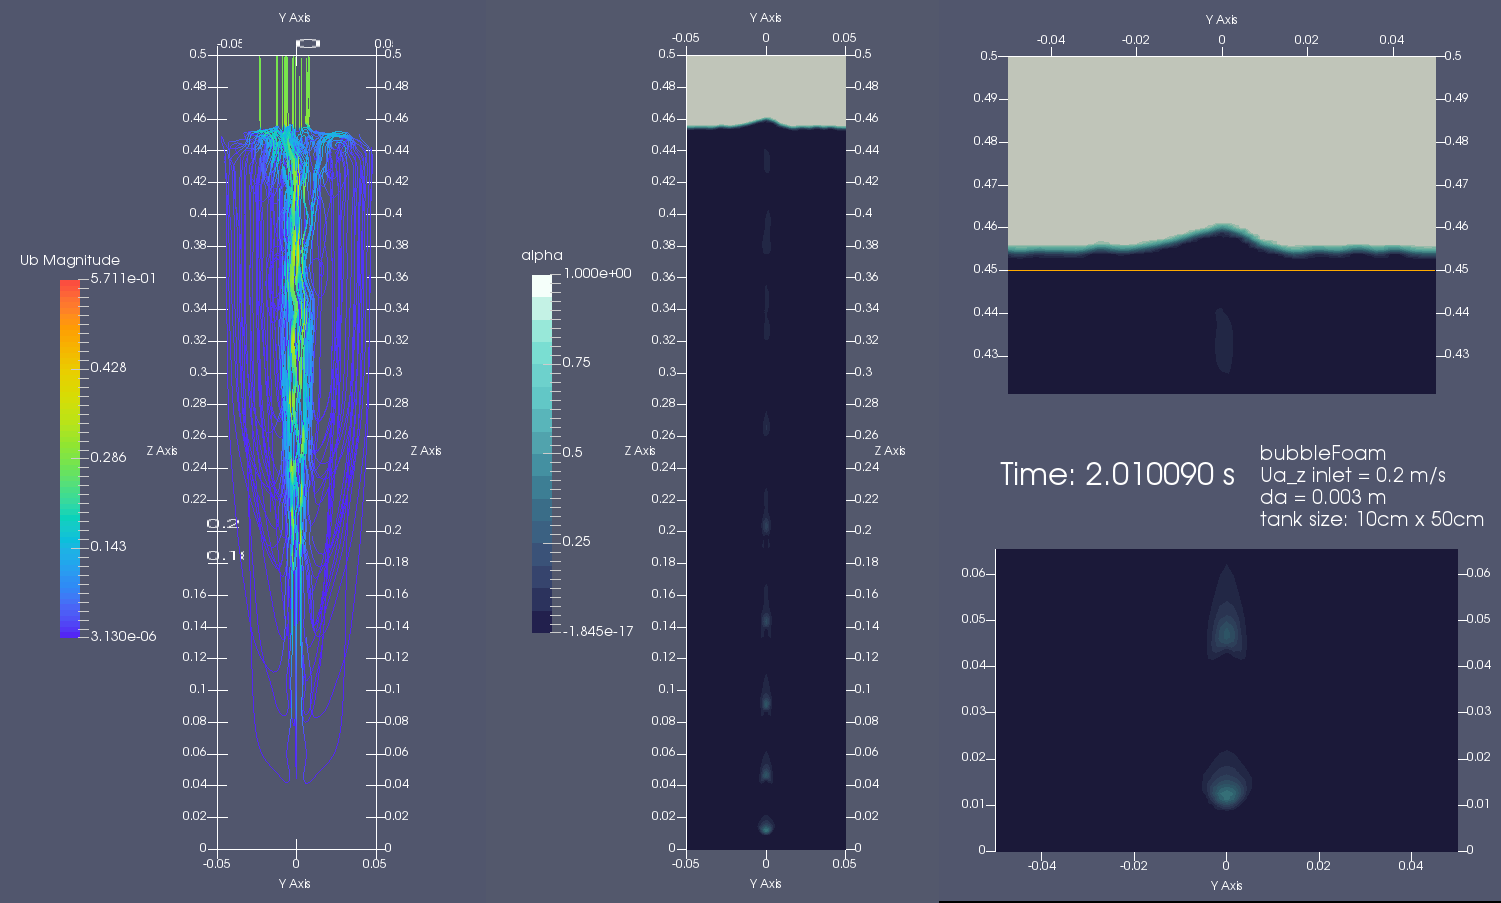
\includegraphics[width=\textwidth]{figures/main/column_streamlines_zoom_da3_Ua02}
    \caption{Continuous phase velocity magnitude and streamlines (left), phase distribution in the column (center) and zoom-in to the top and the bottom part of the column (right) after a quasi-steady state has been achieved. The flow of the distributed phase makes also the continuous phase to move up and, after facing the surface, to recirculate towards the bottom. Formation of individual ``bubble pulses'' is observed, whose size and shape vary as they travel towards the top. The surface level is moved higher than initially set (orange line) and the bubbles interact with the surface. In this scenario, $\SI{3}{\milli\metre}$ air is injected from the bottom with initial velocity of $\SI{0.2}{\metre/\second}$ towards the $z$ direction, once every $\SI{0.08}{\second}$ and with injection duration of $\SI{0.02}{\second}$.}
    \label{fig:main_overview}
\end{figure}

\begin{figure}
    \centering
    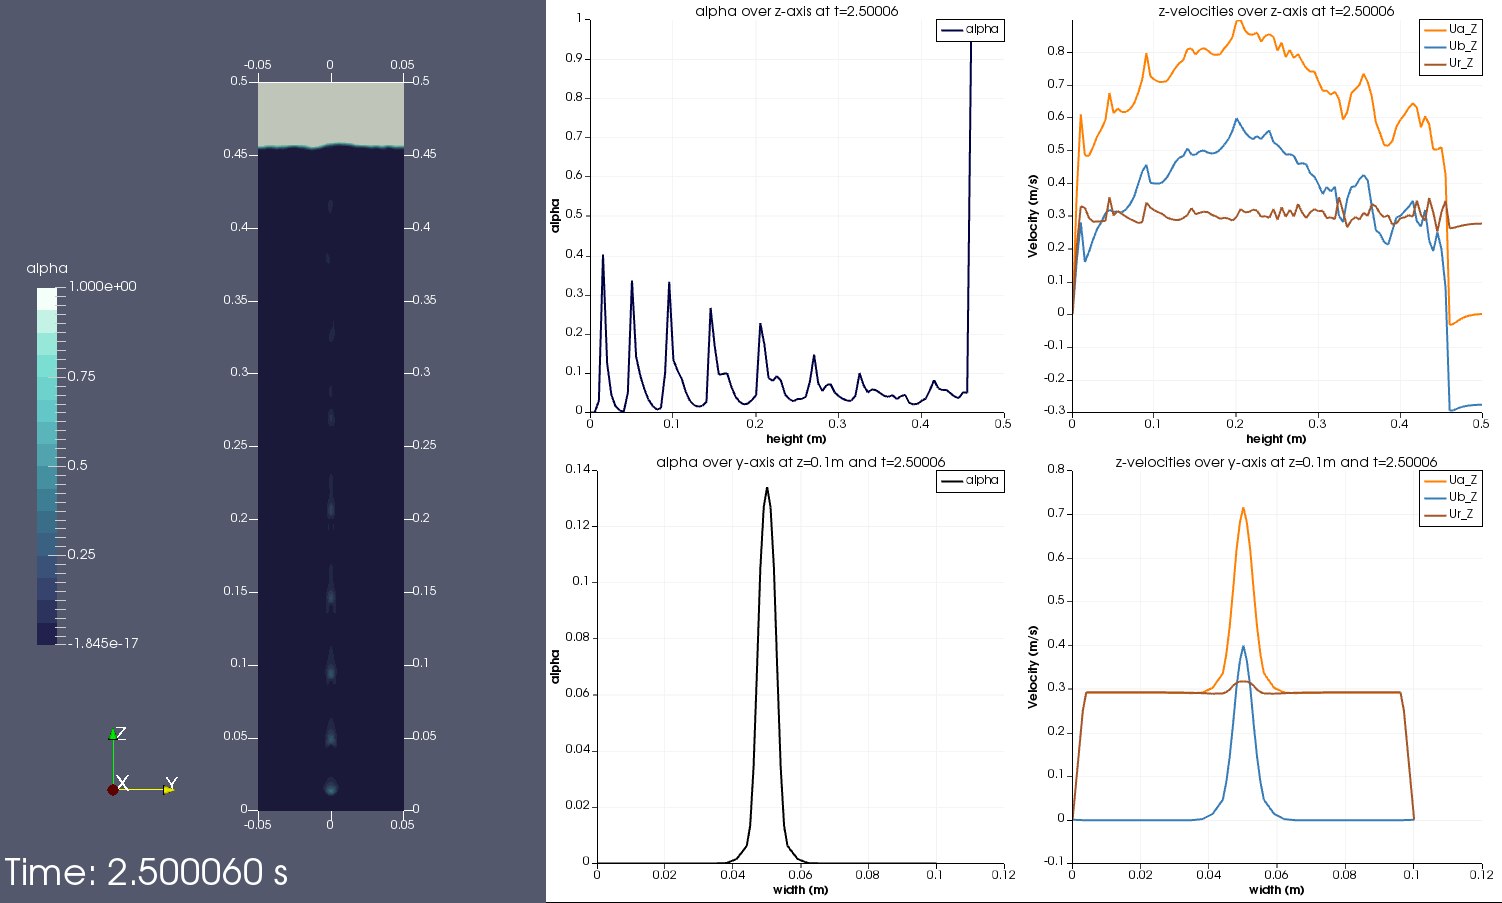
\includegraphics[width=\textwidth]{figures/main/plots}
    \caption{Phase distribution (left) and line plots (center, right) for the main case, at $t=\SI{2.5}{\second}$. \textbf{Top-center:} \texttt{alpha} (gas fraction) distribution across the $z$-axis. Although the area between the individual dispersed phase ``bubbles'' is not completely occupied by the continuous phase, there is a clear distinction between these, that becomes less clear near the top. \textbf{Top-right:} $z$-velocities of the dispersed (\texttt{Ua}, orange) and of the continuous (\texttt{Ub}, blue) phase, as well as relative velocity between the phases (\texttt{Ur}, red). In this quasi-steady state, the phases are accelerated up to a maximum near the middle of the column. After this point, where also the recirculating streamlines shown in figure~\ref{fig:main_overview} start becoming dense, both phases are decelerating. \textbf{Bottom-center:} \texttt{alpha} profile over $y$-axis at $z=\SI{0.1}{\metre}$ and $t=\SI{2.5}{\second}$. The dispersed phase is mainly accumulated in the center axis of the column. \textbf{Bottom-right:} $z$-velocities profiles over the $y$-axis at $z=\SI{0.1}{\metre}$ and $t=\SI{2.5}{\second}$. The dispersed phase is moving faster than the continuous phase and the center of the ``bubble'' is moving faster than both the outer part of the ``bubble'' and the center of the continuous phase.}
    \label{fig:main_plots}
\end{figure}

\begin{figure}
    \centering
    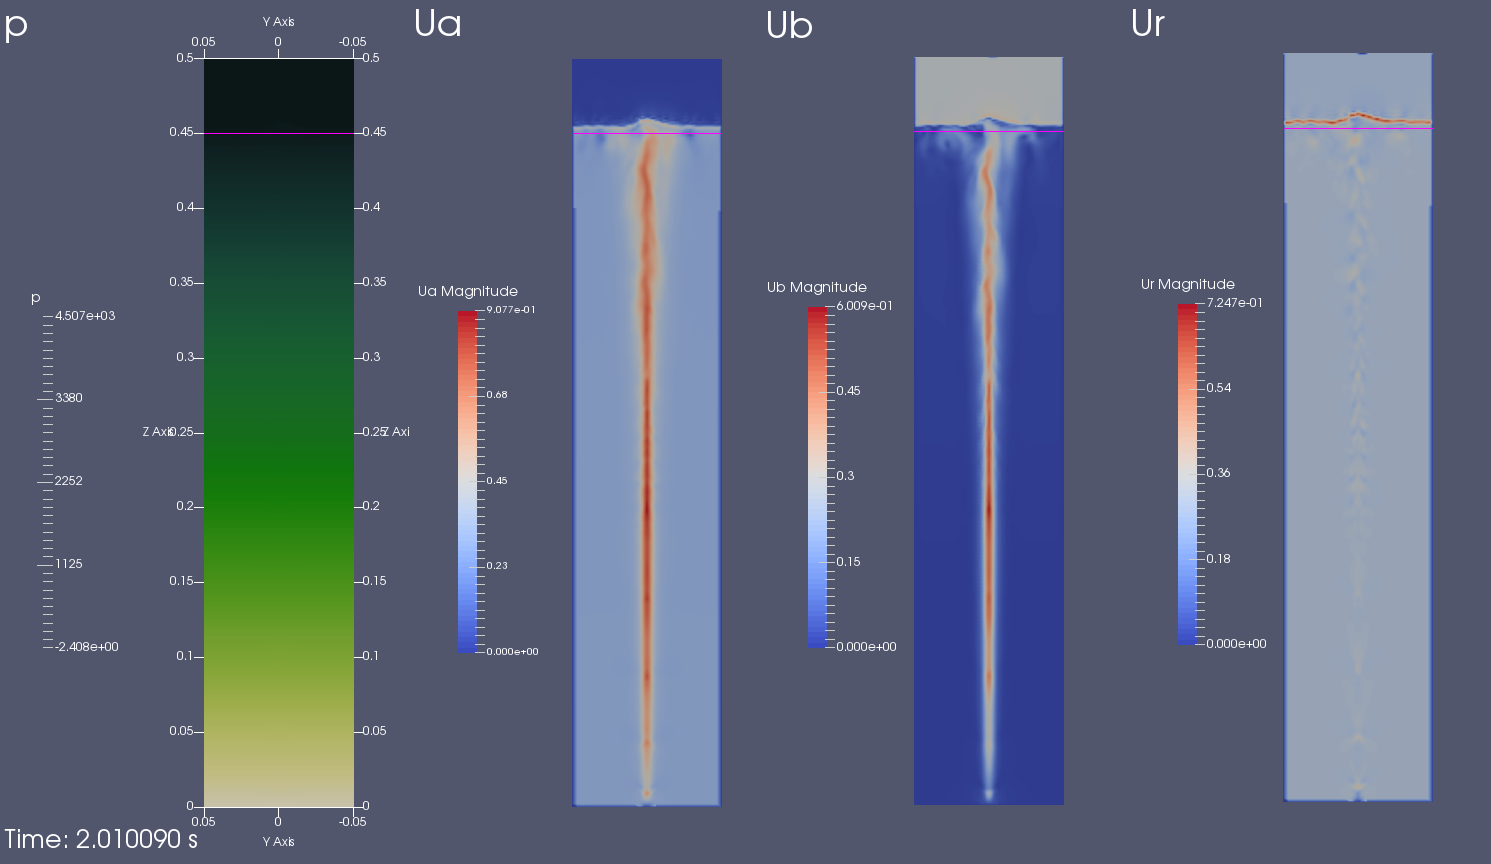
\includegraphics[width=\textwidth]{figures/main/main_p_U}
    \caption{From left to right: pressure, dispersed phase velocity magnitude, continuous phase velocity magnitude and relative velocity magnitude at $t=\SI{2}{\second}$ for the main case. The pink line shows the initial surface level. The higher relative velocity in the center of the bubbles, presented in figure~\ref{fig:main_plots} is also shown here. Please note that the pressure scale colors go from green (low va)ues lto white (high values), as there was a rendering issue with this.}
    \label{fig:main_p_U}
\end{figure}

\begin{figure}
    \centering
    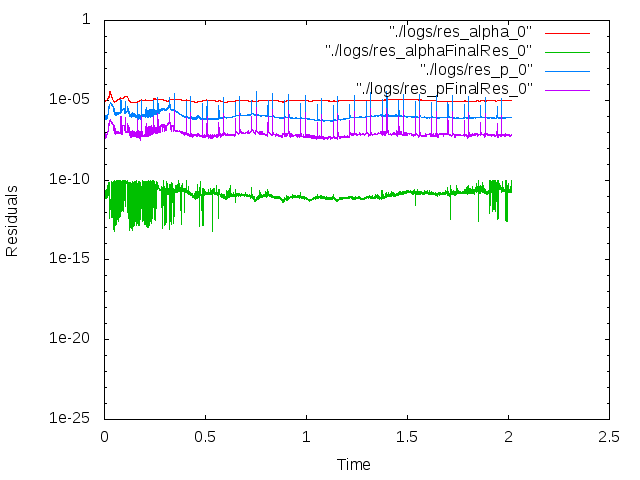
\includegraphics[width=\textwidth]{figures/main/Residuals}
    \caption{Residuals for the main case. The short extremes are expected, due to the periodic injection of bubbles with steep time gradients.}
    \label{fig:main_residuals}
\end{figure}

\subsection{Bubble diameter exploration}
We tested three different values for the dispersed phase diameter, \texttt{da}: $\SI{1}{\milli\metre}$, $\SI{3}{\milli\metre}$ and $\SI{9}{\milli\metre}$. The results after $\SI{1}{\second}$ of simulated time are shown in figure~\ref{fig:main_da_comparison}. We can observe that bigger bubbles arrive at the surface earlier and that smaller bubbles tend to mix together and with the continuous phase more, getting dispersed on the horizontal plane. In figure~\ref{fig:main_da_comparison_Uaz}, the different bubble velocities are depicted, that explain the earlier observation.

\begin{figure}
    \centering
    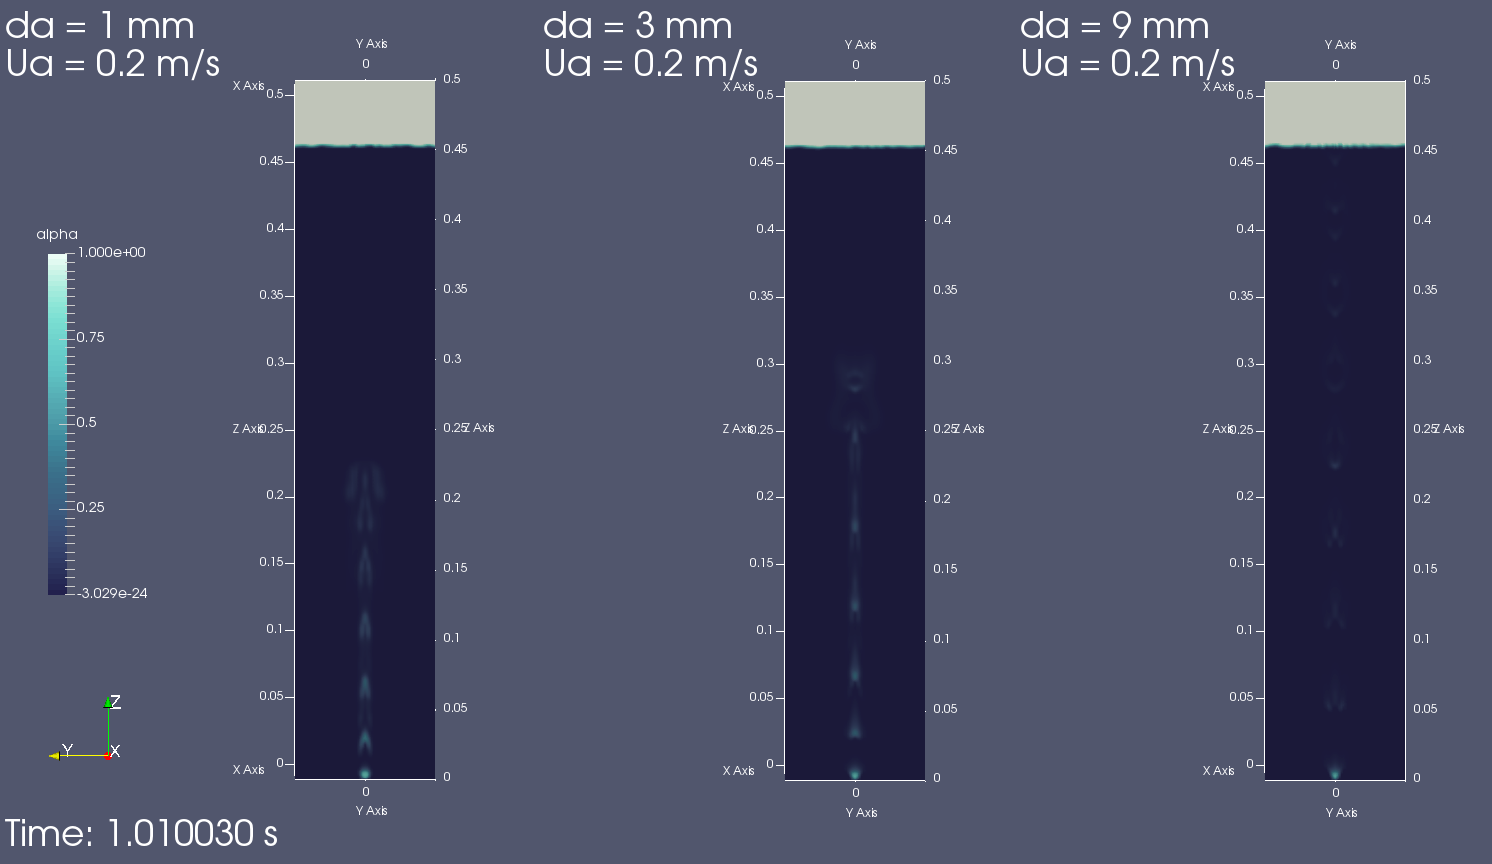
\includegraphics[width=\textwidth]{figures/main/da_comparison_1_3_9}
    \caption{Phase distribution for the main case (center), that sets the diameter of the bubbles to $\SI{3}{\milli\metre}$ and for the same case with $d_\mathrm{a}=\SI{1}{\milli\metre}$ (left) and $d_\mathrm{a}=\SI{9}{\milli\metre}$ (right). In the case of smaller bubbles, the distributed phase areas tend to mix, while in the case of bigger bubbles, these areas tend to stay more distinctive. Also, bigger bubbles travel faster, arriving at the surface level earlier. In all cases, the inlet velocity is set to $\SI{0.2}{\metre/\second}$ and the inlet is a square patch with side $\SI{4}{\milli\metre}$. Different inlet size or finer grid did not change these observations.}
    \label{fig:main_da_comparison}
\end{figure}

\begin{figure}
    \centering
    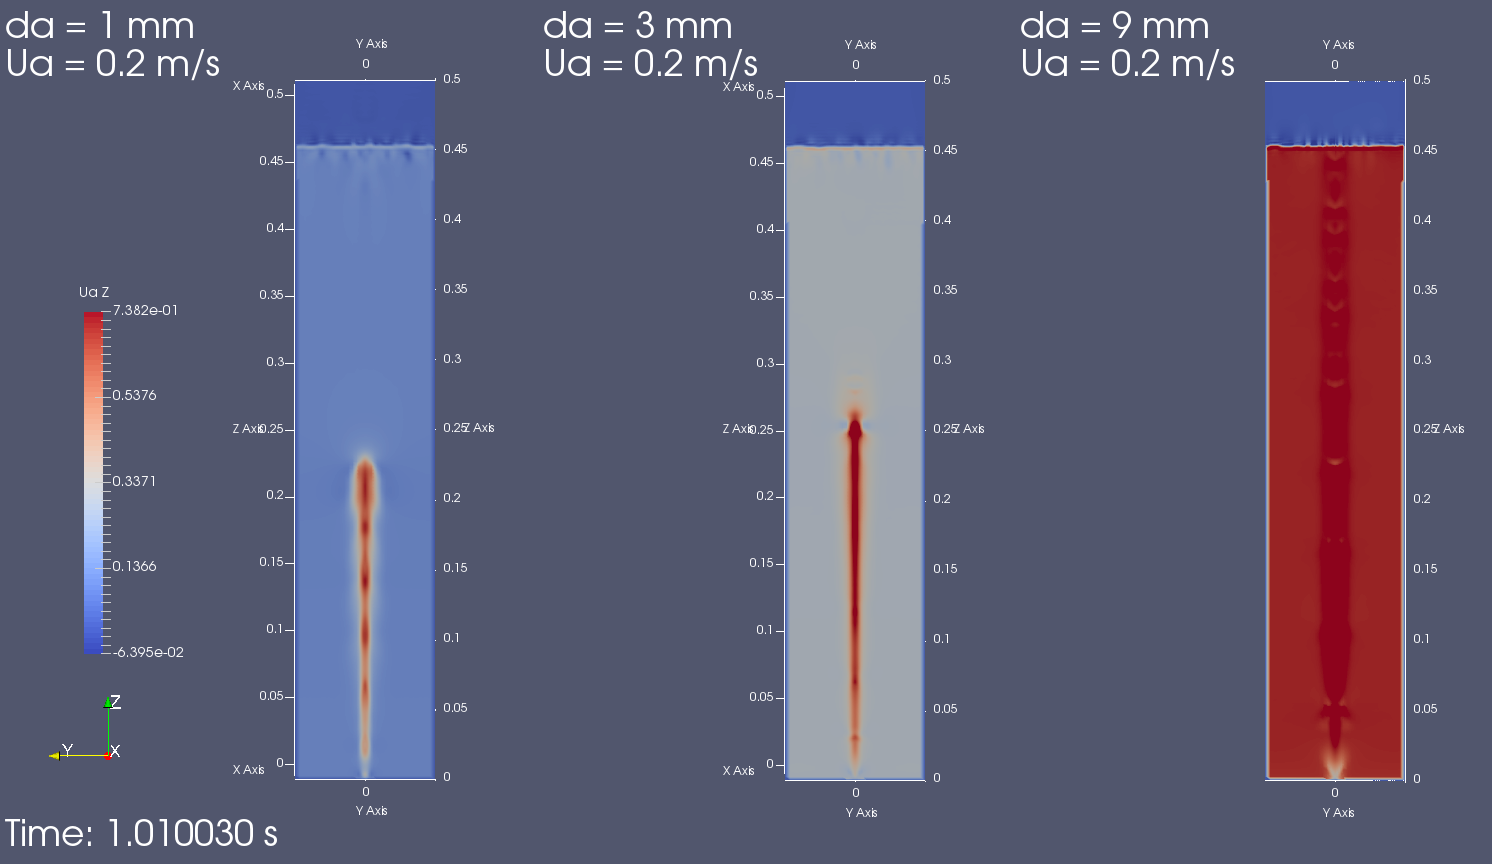
\includegraphics[width=\textwidth]{figures/main/da_comparison_1_3_9_Uaz}
    \caption{Dispersed phase velocity towards the $z$-axis for the main case (center), that sets the diameter of the bubbles to $\SI{3}{\milli\metre}$ and for the same case with $d_\mathrm{a}=\SI{1}{\milli\metre}$ (left) and $d_\mathrm{a}=\SI{9}{\milli\metre}$ (right). The bigger bubbles are traveling with higher velocities in comparison to the smaller. In all cases, the inlet velocity is set to $\SI{0.2}{\metre/\second}$.}
    \label{fig:main_da_comparison_Uaz}
\end{figure}

\subsection{Inlet velocity exploration}
Apart from different bubble diameters, we also tested different air velocities at the inlet. We tested the values of $U_{\mathrm{a},z} = \SI{0.07}{\metre/\second}$, $\SI{0.2}{\metre/\second}$ and $\SI{0.6}{\metre/\second}$. The distribution of the bubble areas in the column changes, with lower-speed bubbles tending to stay together, while higher-speed bubbles tend to mix with the continuous phase. We also observe that higher velocity at the inlet gives also higher air velocity inside the column, as well as higher velocity of the continuous phase, as expected. The results are shown in figures~\ref{fig:main_Ua_comparison}, \ref{fig:main_Ua_comparison_Uaz} and~\ref{fig:main_Ua_comparison_Ubz}.

\begin{figure}
    \centering
    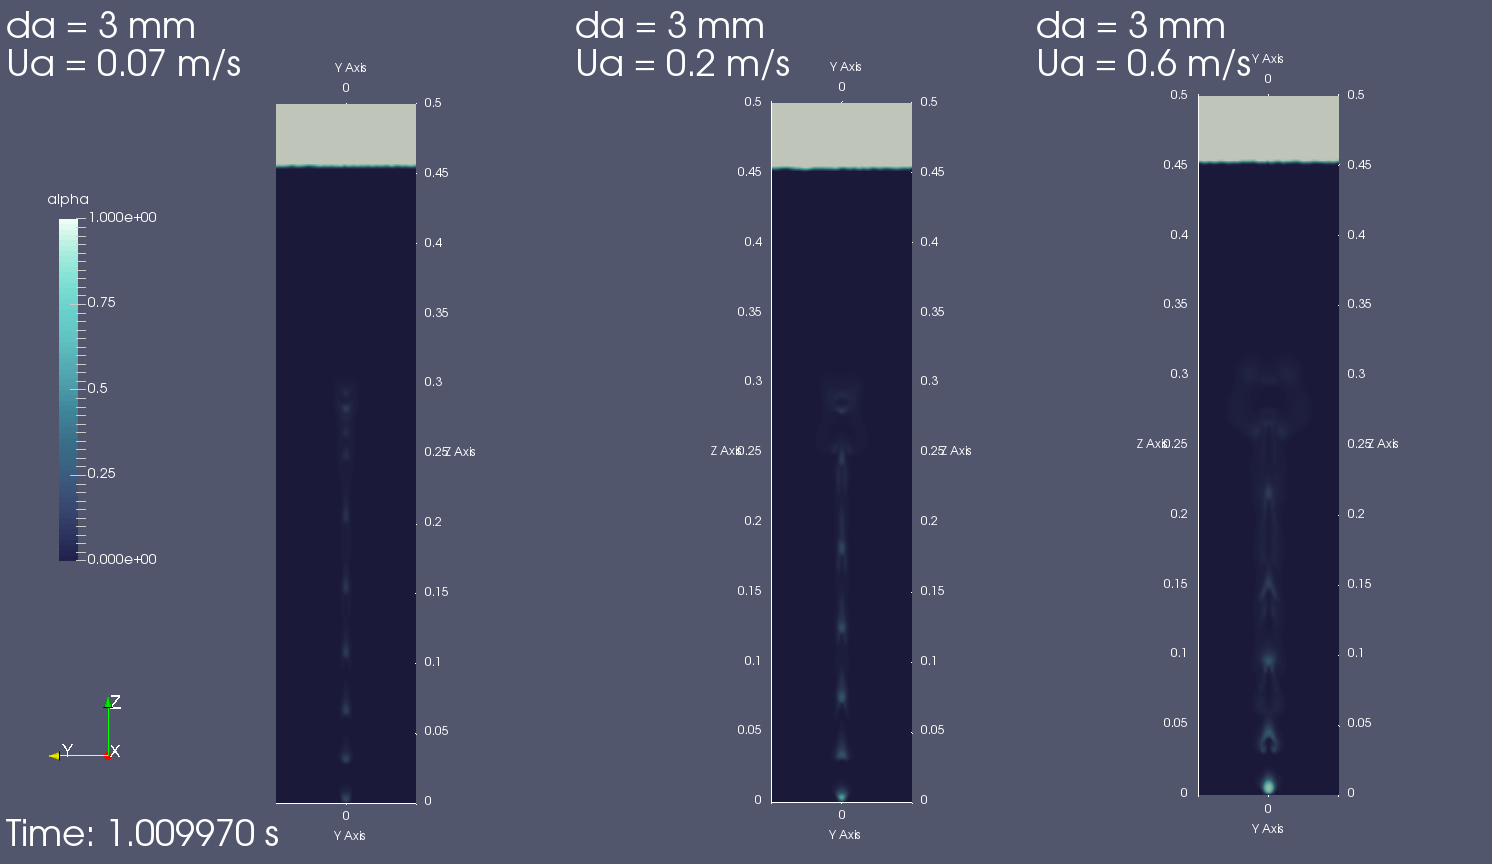
\includegraphics[width=\textwidth]{figures/main/Ua_comparison}
    \caption{Phase distribution for the main case (center), that sets the inlet velocity of the air towards $z$ to $\SI{0.3}{\metre/\second}$ and for the same case with $U_{\mathrm{a},z}=\SI{0.07}{\metre/\second}$ (left) and $U_{\mathrm{a},z}=\SI{0.6}{\metre/\second}$ (right). When the air is injected with lower velocity, the bubble areas stay together, while in higher inlet velocities it tends to mix with the continuous phase. In all the cases, \texttt{da} is set to $\SI{3}{\milli\metre}$.}
    \label{fig:main_Ua_comparison}
\end{figure}

\begin{figure}
    \centering
    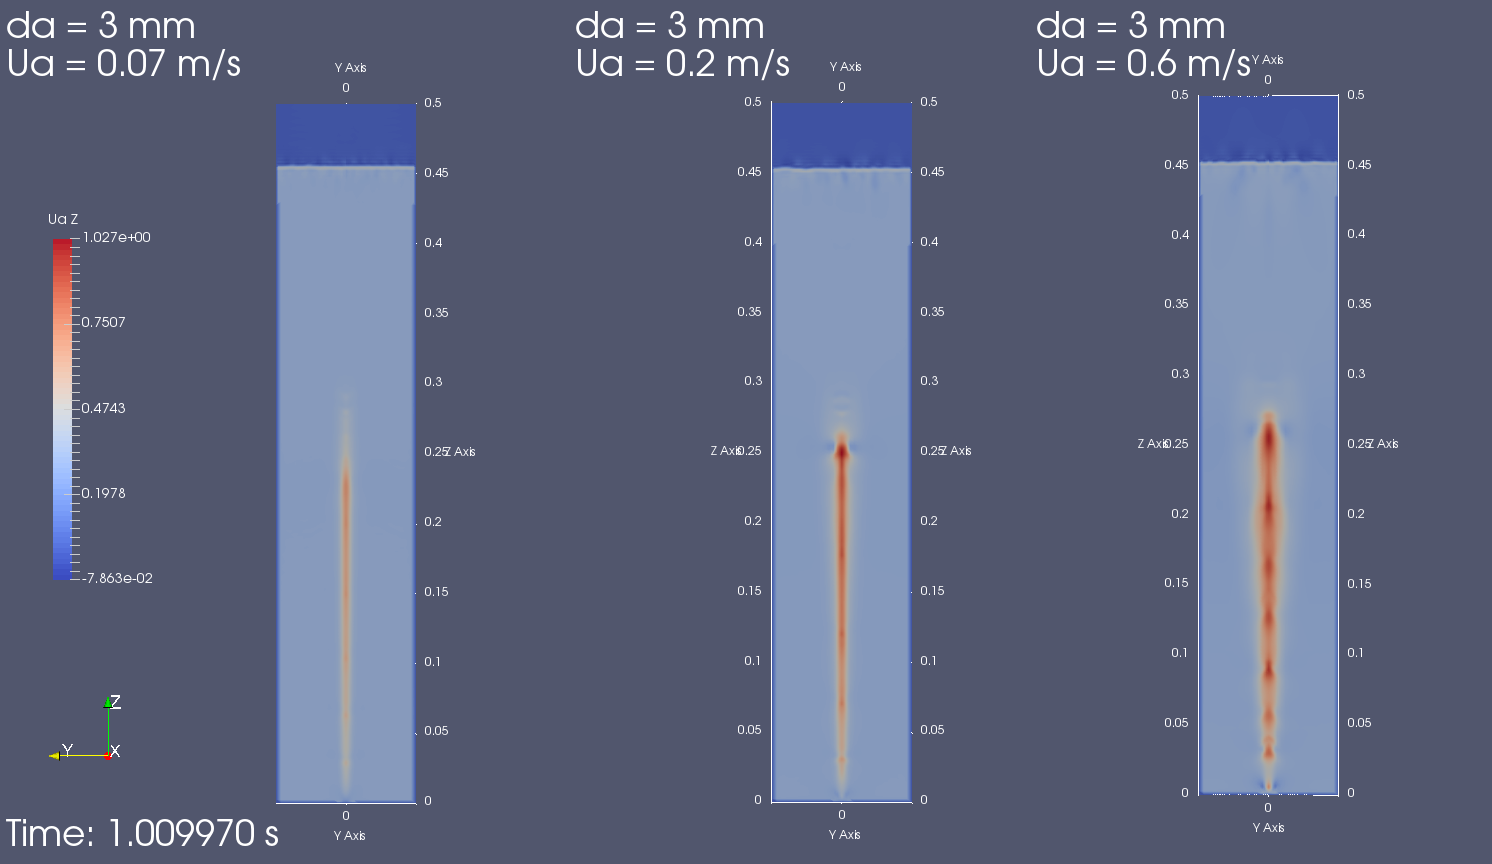
\includegraphics[width=\textwidth]{figures/main/Ua_comparison_Uaz}
    \caption{Dispersed phase velocity towards $z$ for the main case (center), that sets the inlet velocity of the air towards $z$ to $\SI{0.3}{\metre/\second}$ and for the same case with $U_{\mathrm{a},z}=\SI{0.07}{\metre/\second}$ (left) and $U_{\mathrm{a},z}=\SI{0.6}{\metre/\second}$ (right). Higher inlet velocity leads also to higher air velocity inside the column. In all the cases, \texttt{da} is set to $\SI{3}{\milli\metre}$.}
    \label{fig:main_Ua_comparison_Uaz}
\end{figure}

\begin{figure}
    \centering
    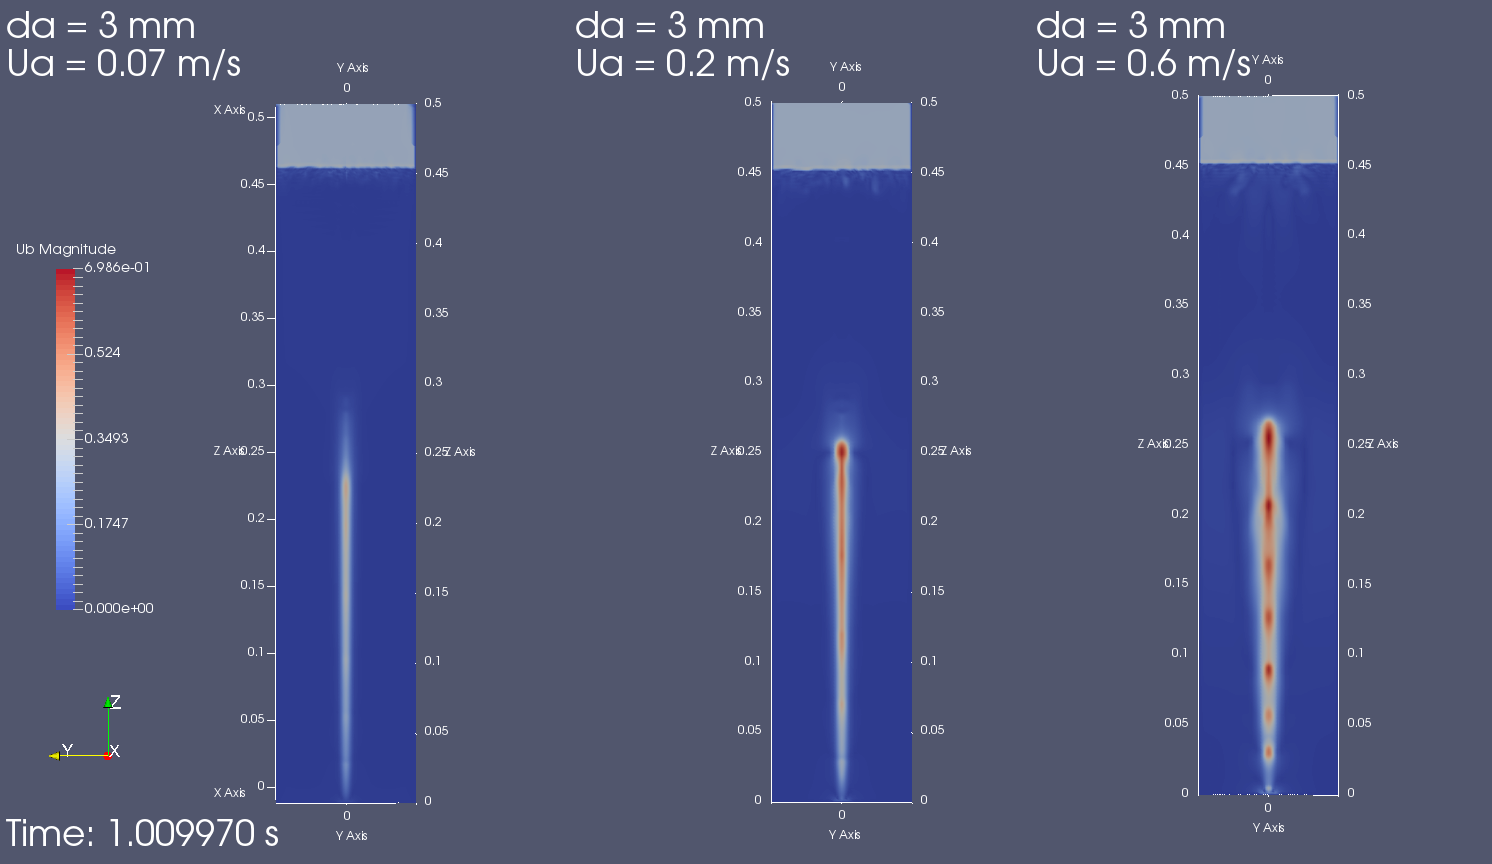
\includegraphics[width=\textwidth]{figures/main/Ua_comparison_Ubz}
    \caption{Continuous phase velocity towards $z$ for the main case (center), that sets the inlet velocity of the air towards $z$ to $\SI{0.3}{\metre/\second}$ and for the same case with $U_{\mathrm{a},z}=\SI{0.07}{\metre/\second}$ (left) and $U_{\mathrm{a},z}=\SI{0.6}{\metre/\second}$ (right). Higher inlet velocity leads also to higher velocity inside for the continuous phase. In all the cases, \texttt{da} is set to $\SI{3}{\milli\metre}$.}
    \label{fig:main_Ua_comparison_Ubz}
\end{figure}

\subsection{Interaction with obstacles}
Following the main scenario, we introduced an obstacle to study how the dispersed phase behaves after it. On the one hand, this would give us some insight on the capabilities of the solver. On the other hand, this is a problem with industrial interest, as obstacles are sometimes used to break big bubbles to smaller in bioreactors. The results are shown in the figures~\ref{fig:obstacle_overview} and~\ref{fig:obstacle_colored}.

In figure~\ref{fig:obstacle_overview} the geometry and mesh are shown, as well as the separation of big bubble areas to smaller. In figure~\ref{fig:obstacle_colored} we observe that these smaller areas have the form of rings (most of the time). Interestingly, in the very first moments of the evolution, a big square is formed on the surface, related to the shape of the inlet hole (not shown here, see the animations).

\begin{figure}
    \centering
    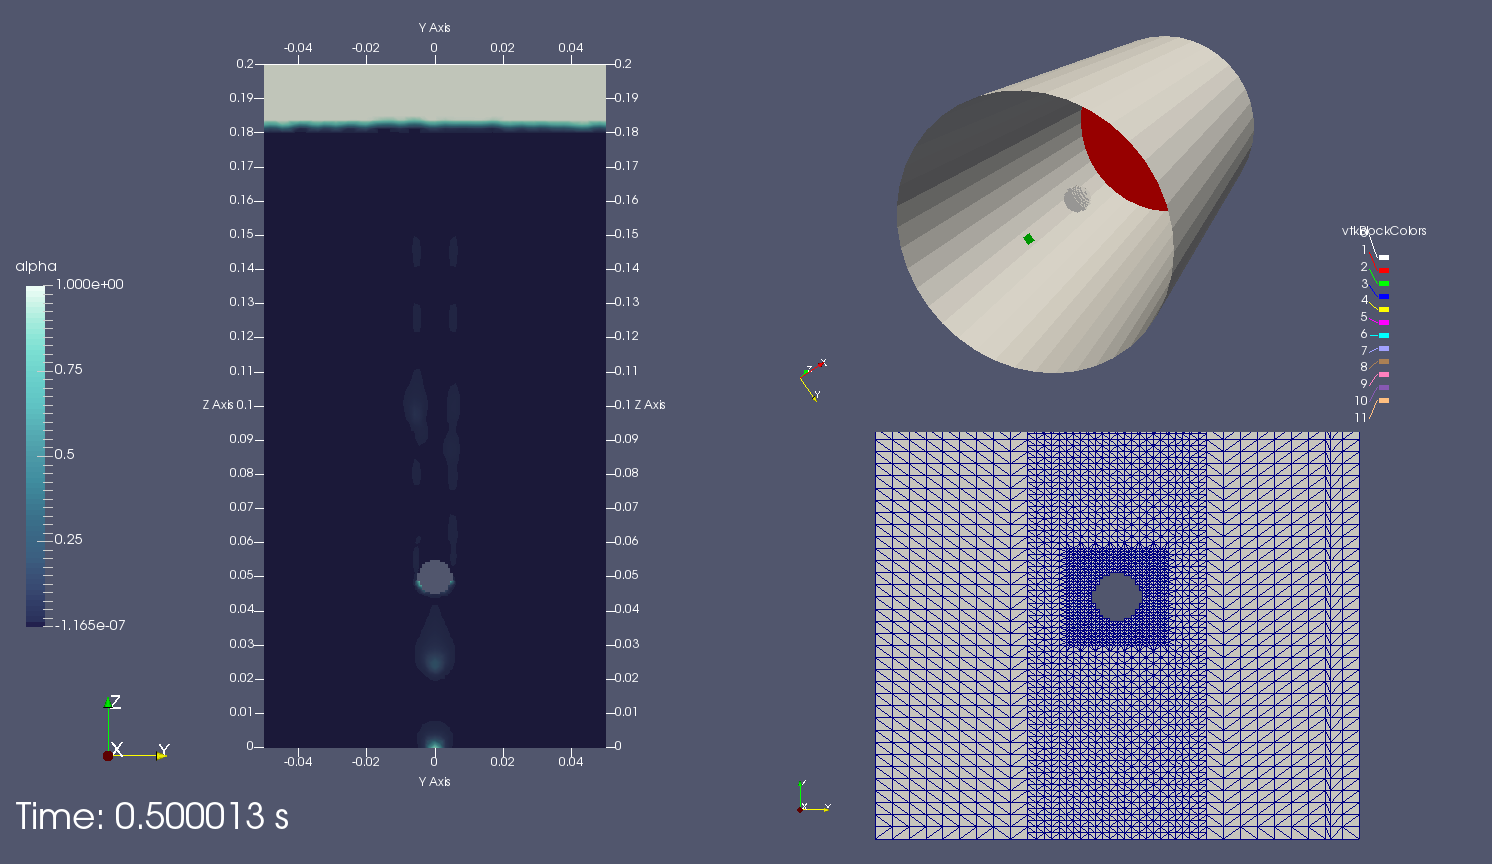
\includegraphics[width=\textwidth]{figures/obstacle/obstacle}
    \caption{Interaction with an obstacle. \textbf{Left:} phase distribution. After colliding on the spherical object, the dispersed phase area is divided to two areas. \textbf{Right-top:} geometry of the scenario. The spherical obstacle is a part of the wall boundaries and it is aligned above the inlet. \textbf{Right-bottom:} Apart from the first stage of refinement, applied also in the main case (figure~\ref{fig:main_mesh}), a second level of refinement is applied around the obstacle. No surface-fitting was applied around the obstacle.}
    \label{fig:obstacle_overview}
\end{figure}

\begin{figure}
    \centering
    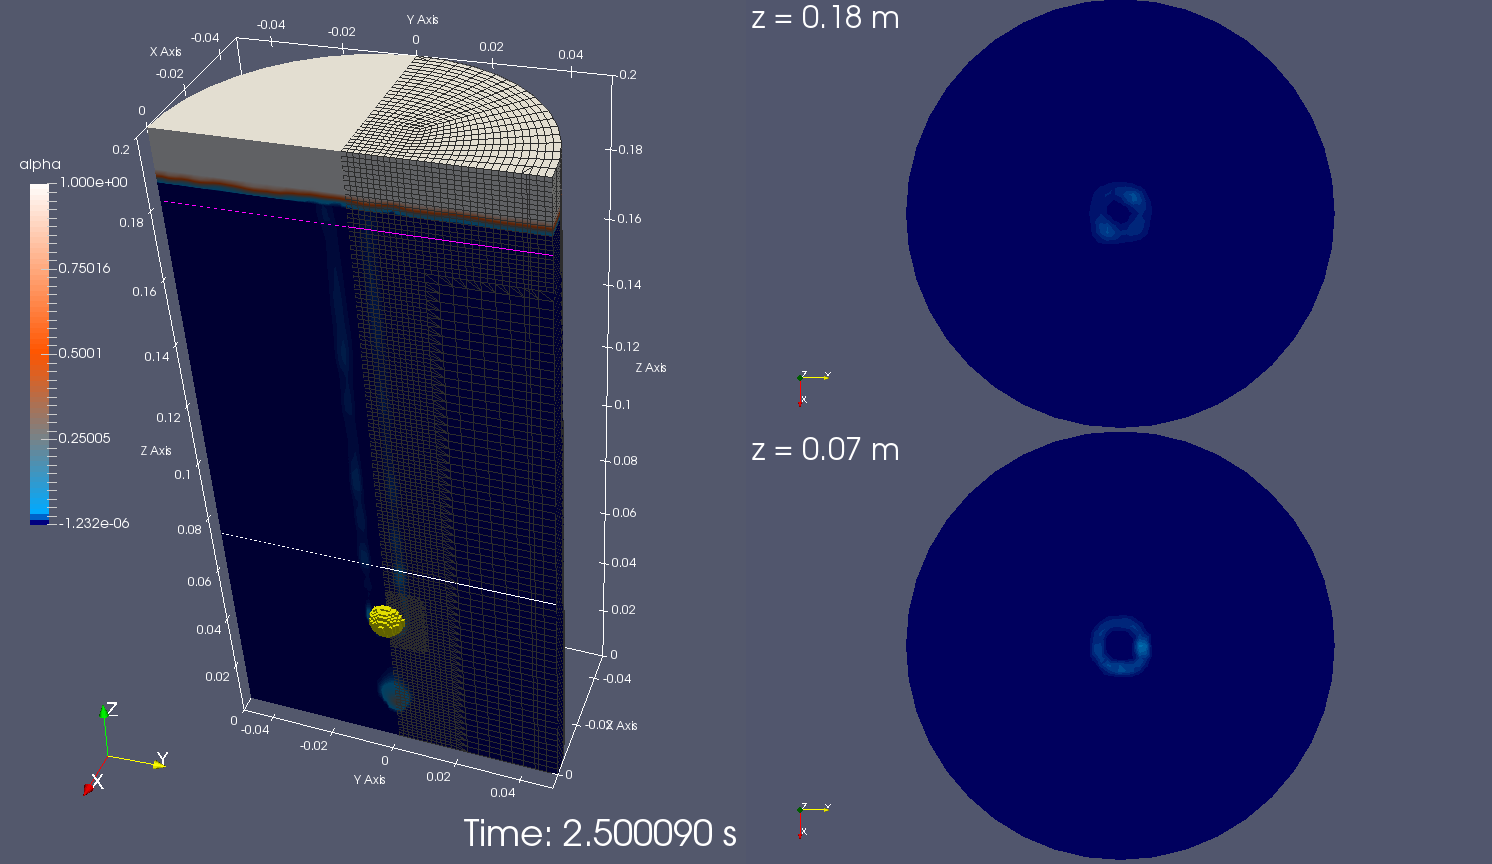
\includegraphics[width=\textwidth]{figures/obstacle/obstacle_3D_slices}
    \caption{Interaction with an obstacle, 3D view and slices at $z=\SI{0.07}{\metre}$ (bottom) and $z=\SI{0.18}{\metre}$ (initial surface level, top). The colors are adjusted to better visualize the dispersed phase volume breakage. After the obstacle, the dispersed phase forms rings.}
    \label{fig:obstacle_colored}
\end{figure}

\subsection{Solver aspects}
Some interesting problems and observations arose during our early experiments. In figure~\ref{fig:square_to_round} an early low-velocity scenario is shown, with long air injections. Taking two slices on different height locations, we observe that the cross-section of the bubble has initially the shape of the square inlet. The shape changes to round as the bubble travels towards the surface. This hints us that the solver takes into account the surface tension and/or the pressure effects on the dispersed phase.

On figure~\ref{fig:numerical_diffusion} another problem that was observed in low-velocity scenarios with coarse grids is shown. In order to visualize bubbles in so small \texttt{alpha} values, very low thresholds are set, that allow us to observe the problem. Due to numerical issues, the outer cells of the inlet, in which the gradient is high, tend to give higher \texttt{alpha} values. This accumulates over time and looks like a (false) diffusion. The result is this unphysical, sharp face of the bubble.

On figure~\ref{fig:twoPhaseEulerFoam} \texttt{bubbleFoam} is compared to the newer \texttt{twoPhaseEulerFoam}, that is used in other studies. Overall the two solvers give very similar results. A case of difference is shown here, where the \texttt{twoPhaseEulerFoam} seems to not interact with the surface in the same magnitude. The shown peak is getting higher over time, as more bubbles arrive, until it collapses. The shape of the bubbles is also a bit different on the bottom. Although the same parameters of \texttt{bubbleFoam} have been used in the \texttt{twoPhaseEulerFoam}, there are also some extra parameters that may affect the solution. They were set the same as in the provided tutorial.

\begin{figure}
    \centering
    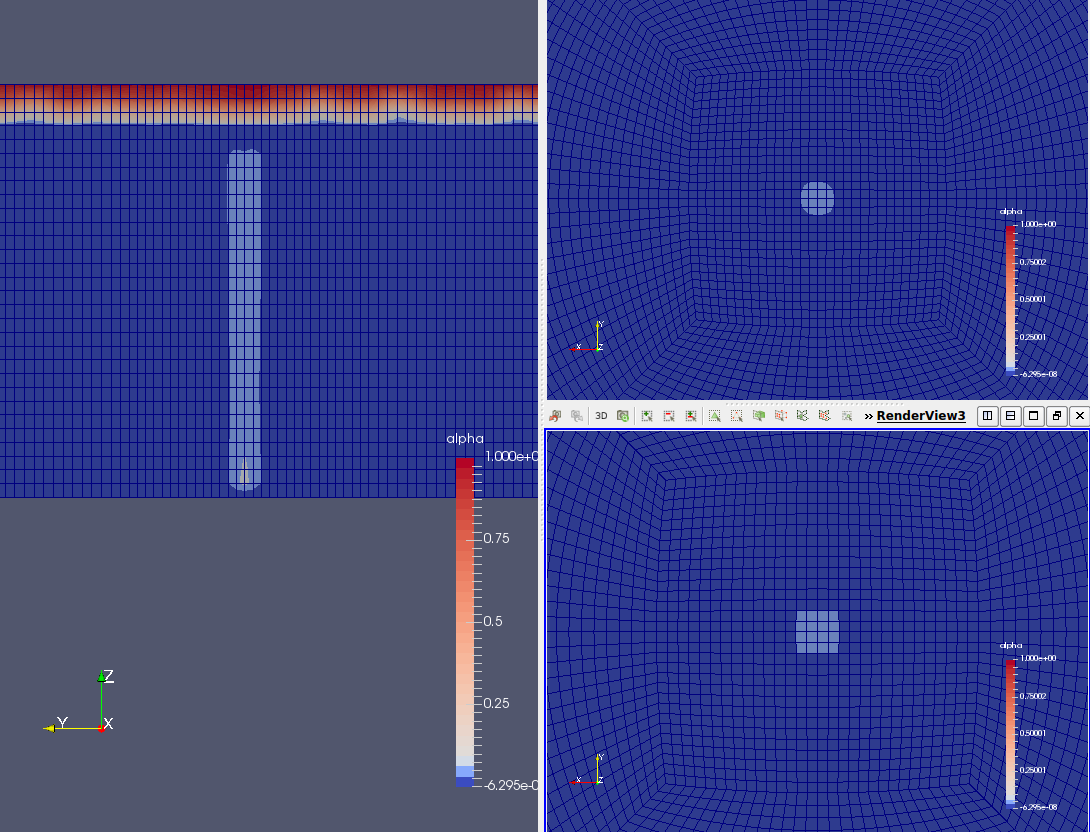
\includegraphics[width=\textwidth]{figures/square_to_round_early}
    \caption{Early results with far from optimal parameters. In this low-velocity scenario ($\SI{0.01}{\metre/\second}$, once every $\SI{0.1}{\second}$ and for $\SI{0.05}{\second}$), the gradual transformation of the bubble cross-section from a perfect square (right-bottom) to a circle (right-top), as it travels towards the surface, can be observed. In our main case, this happens instantly and the gradual transformation cannot be observed. Note that the color scale has been adjusted to visualize the air-rich areas more clearly.}
    \label{fig:square_to_round}
\end{figure}

\begin{figure}
    \centering
    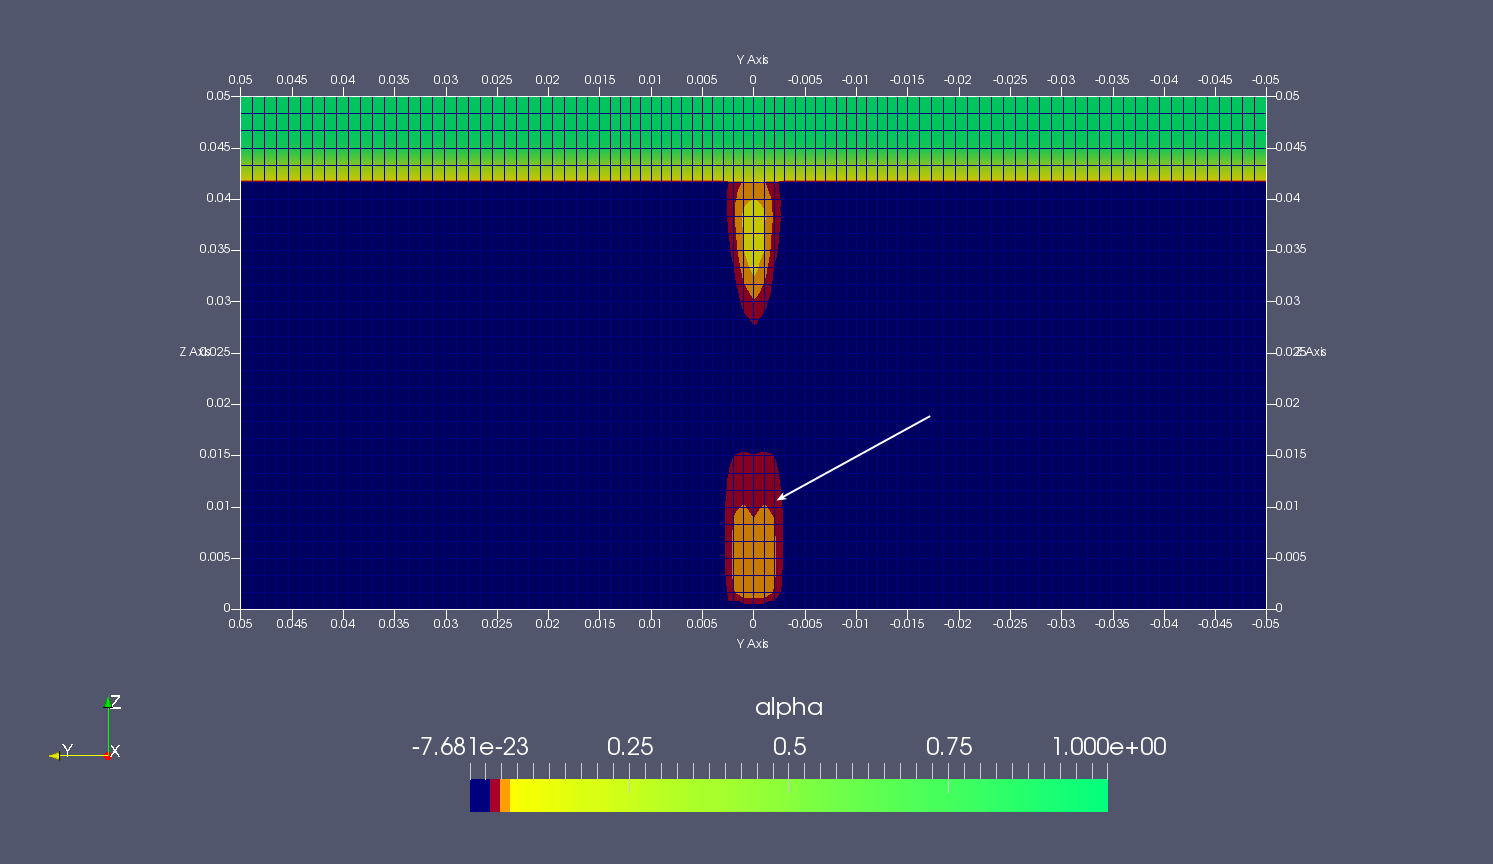
\includegraphics[width=\textwidth]{figures/early_numerical_diffusion_annotated}
    \caption{Similar early results as in figure~\ref{fig:square_to_round}. In order to visualize bubble areas, the color scale needed to be shifted towards very low \texttt{alpha} values. In these low values, numerical diffusion is observed, as the Volume-Of-Fluid method is used. Steep gradients are also introduced around the inlet, as the \texttt{Ua} is set uniformly for the respective inlet cells. Notice the sharp-edged shape of the injected bubble area. This was cured by increasing the inlet velocity and refining the mesh, therefore increasing the \texttt{alpha} values near the inlet.}
    \label{fig:numerical_diffusion}
\end{figure}

\begin{figure}
    \centering
    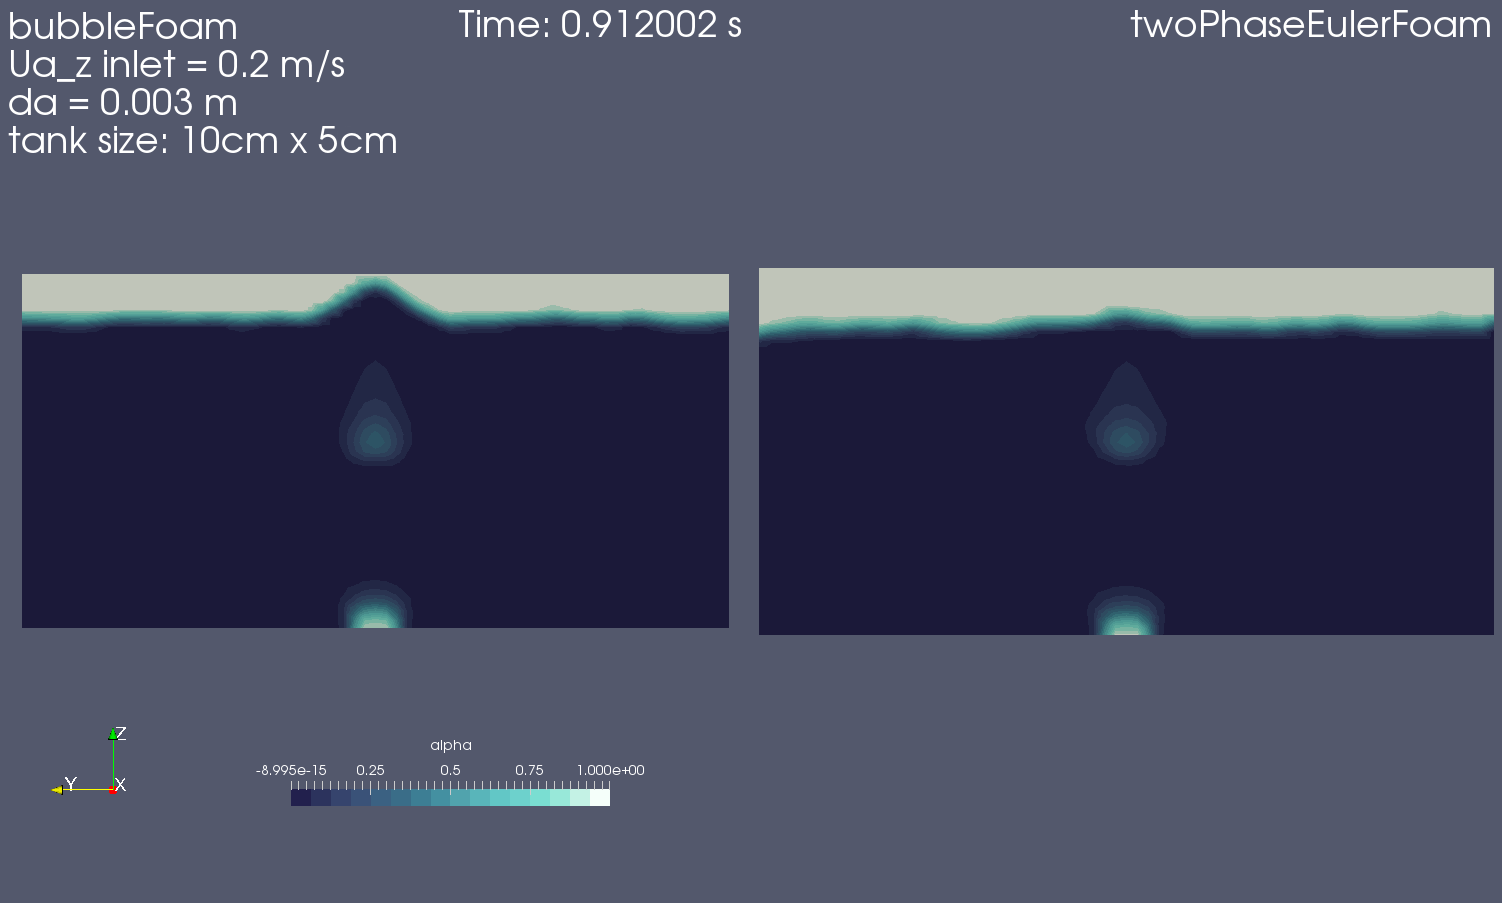
\includegraphics[width=\textwidth]{figures/bubbleFoam_vs_twoPhaseEulerFoam}
    \caption{Comparison between the \texttt{bubbleFoam} and the newer \texttt{twoPhaseEulerFoam}. The \emph{bubbleColumn} tutorial of each solver was used as a base, adapted to fit our approach. The same parameters of \texttt{bubbleFoam} were used in the \texttt{twoPhaseEulerFoam} case, although the latter takes also some extra parameters. The \texttt{bubbleFoam} affects more the surface, while the \texttt{twoPhaseEulerFoam} provides a rounder bubble volume. The observed peak is increasing in height over time and it collapses after a maximum.}
    \label{fig:twoPhaseEulerFoam}
\end{figure}

\section{Conclusion}
% { Achievement of the goals? Problems encountered? }

\subsection{Lessons learned}
The figure~\ref{fig:overview} summarizes the tools we used at each step of our project. Overall, we combined several tools that we first used in the previous exercises, and we used some others for the first time, like the \texttt{bubbleFoam} and \texttt{twoPhaseEulerFoam} solvers, the \texttt{timeVaryingUniformFixedValue} boundary condition, the \texttt{sphereToCell} selection function and the \texttt{arc} type of edges in \texttt{blockMeshDict}. We didn't add any custom source code, as we tried to do everything with tools that were already available and therefore more generic and portable. We also used \texttt{Paraview} extensively, in order to better visualize our results.

We simulated a 3D bubble column scenario and we were able to observe the main phenomena that we expected, as well as some that we were not aware of before. Expected observations were the rising of the surface level, the water flow induced by the air flow, the interaction with the surface and the decrease in the size of the ``bubbles'' as they travel towards the top. We saw a clear dependency of the bubbles shape and velocity on their size and on the inlet conditions. We also observed the expected breakage of the bubble areas when they faced an obstacle. More interesting were the evolution of the bubble shape and especially the strong drag and lift effects that made the bubbles sharper, as well as their deceleration near the top. A nice addition to that was the strong cross-section transformation of the bubbles as they leave the square inlet hole.

Exploring the range of parameters in order to get results close to our physical expectations, we faced some problems and we better understood some numerical aspects. Since the beginning, we faced the challenge of simulating a big domain in feasible time and we learned that it is better to build the domain step-by-step. Therefore, we ran our first simulations with less cells, or on shorter columns with the same cell density. We were also assisted by the parallel execution feature of OpenFOAM, that in our problem was seamlessly configured. Some of the numerical issues that we faced was the selection of an appropriate timestep size for a stable solution, something that was solved using an adaptive timestep, bounded by the Courant number. We also saw that numerical diffusion is an important issue and we found some ways to heal it.

\begin{figure}
    \centering
    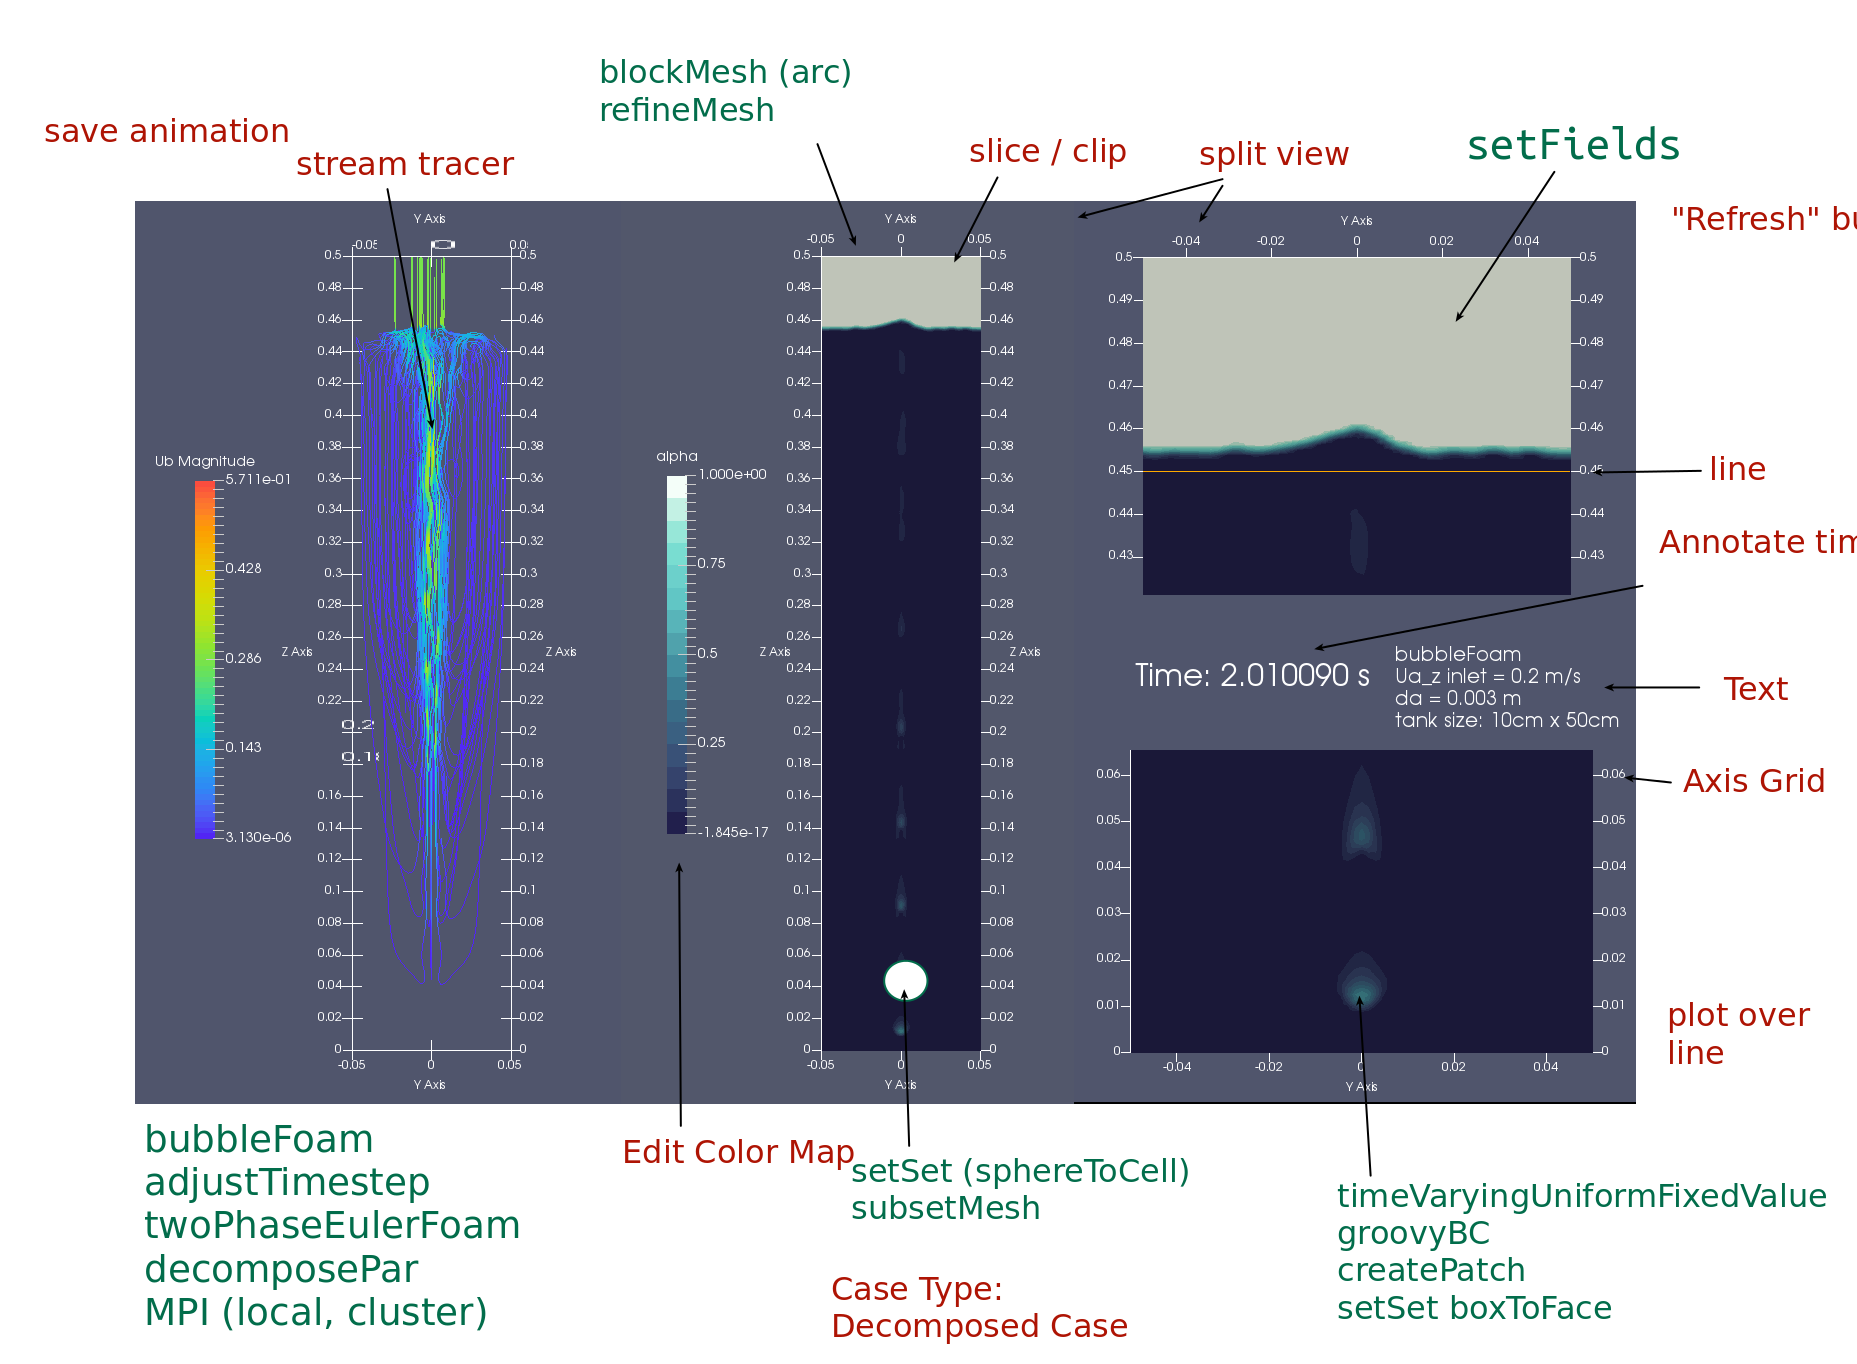
\includegraphics[width=\textwidth]{figures/overview}
    \caption{Overview of the tools used in this project.}
    \label{fig:overview}
\end{figure}

\subsection{Future work}
This project gave us an overview of how a bubble column simulation can be set and what aspects of the simulation are challenging. It helped us better understand the phenomena behind it, but it also opened many questions and ideas for further studies. The following would be interesting for us or maybe for other students too in the future:
\begin{enumerate}
    \item Add more bubble injection points. This would require changes in the mesh and it would give us a better understanding of the complex phase interactions inside an actual bubble column. An inclusion of a range of phase diameters would also be a more realistic modelling approach.
    \item Use a more advanced multiphase solver to study the phase interaction in better depth. Phenomena as heat and mass exchange could be added. An additional phase could be added, e.g.\@ an oil phase, that could correspond to biomass. In that case, modelling of chemical reactions would be very interesting. There are several newer related solvers introduced in the newer versions of OpenFOAM, that include these features.
    \item Add more obstacles and complex geometries. This would require the design of the geometry in a CAD software, conversion to OpenFOAM and adaption of the mesh. Objectives could be the maximization of the contact time between the two phases or the gradual breakage of big bubbles to finer. Systems like these are used, for example, in the aeration stage of wastewater treatment.
    \item Add particle tracking. This could correspond to light solids that also exist in some of the related industrial problems.
\end{enumerate}


% \nomplex geometriecite{*}
% \printbibliography

\end{document}


%%%% Examples

% Code listing

% \begin{lstlisting}[language=C++, caption={}, label={lst:}]
%
% \end{lstlisting}


% Tables using the "tabular" package. No text wrapping available.

% \begin{table}
% \centering
% \begin{tabular}{c|cc}
% \hline
% \textbf{Fields} & \textbf{Initial v.} & \textbf{Wall}\\
% \hline    
%      &   &  \\
% \hline
% \end{tabular}
% \caption{}
% \label{tab:}
% \end{table}


% Tables using the "tabulary" package. Some cells can allow text wrapping (use L,R,C instead of l,r,c). You can force a line break with \newline.

% \begin{table}
% \centering
% \begin{tabulary}{\linewidth}{l|lLlL}
% \hline
% \textbf{Fields} & \textbf{Initial} & \textbf{Inlet} & \textbf{Outlet} & \textbf{Wall}\\
% \hline    
%     Velocity, U & (0 0 0)  & fixedValue\newline (0 0.005 0) & zeroGradient & fixedValue\newline (0 0 0)\\
%     \hline
%     Pressure, p & 0        & zeroGradient           & fixedValue 0 & zeroGradient      \\
% \hline
% \end{tabulary}
% \caption{Initial and boundary conditions for the main case.}
% \label{tab:case_main}
% \end{table}


% Figures

% \begin{figure}
%     \centering
%     \includegraphics[width=\textwidth]{figures/}
%     \caption{}
%     \label{fig:}
% \end{figure}